\documentclass[]{article}
\usepackage{listings} 
\usepackage{algorithm}
\usepackage{algorithmic}
\usepackage{graphicx}
\graphicspath{ {images/} }
\usepackage{float}
\usepackage{geometry}
\usepackage{pdfpages}

%opening
\title{}
\author{}
\date{}
\special{papersize=8.5in,11in}
\geometry{left=1.5cm,right=2cm,top=1.5cm,bottom=1.5cm}

\begin{document}
	
	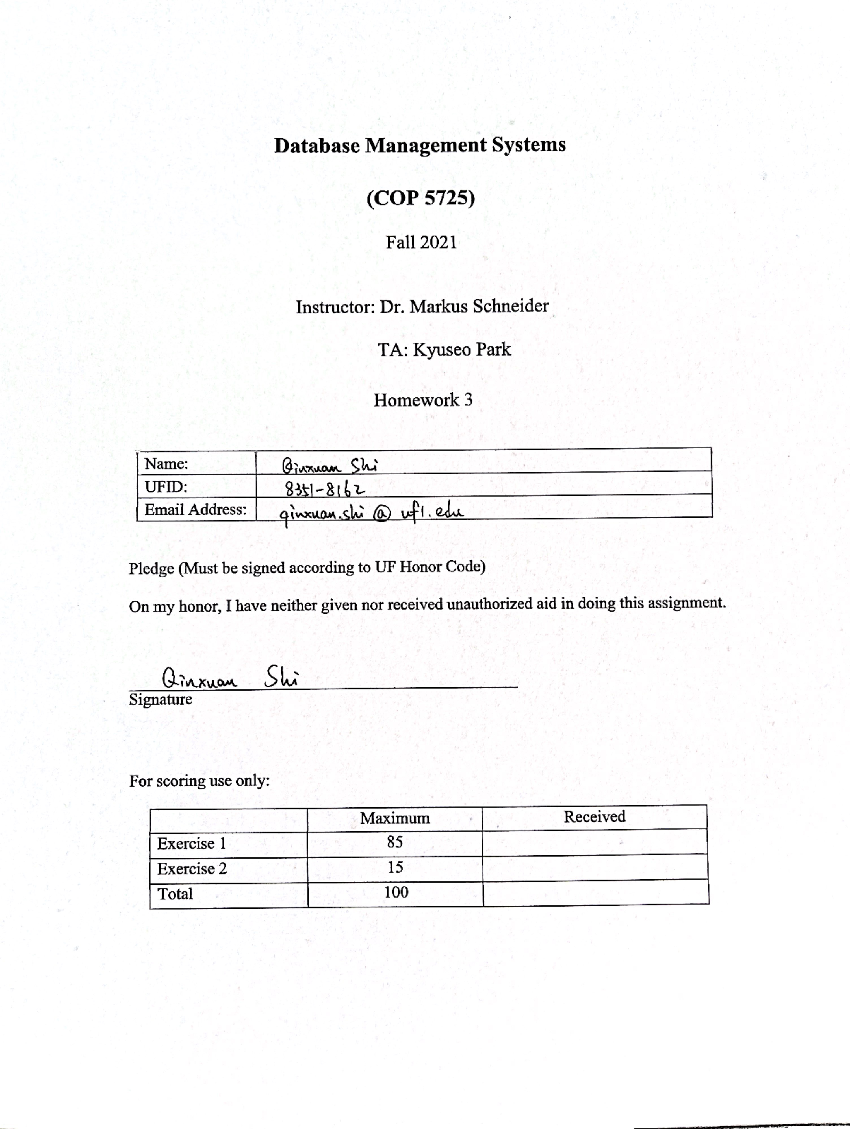
\includepdf{../HW3.pdf}
	
	\section{Exercise 1}
	
	\subsection{explore scenario}
	
	1. What is the meaning of these keywords?  \\
	
	\noindent The latter [NOT DEFERRABLE] is default, and means that every time a database modification statement is executed, the constraint is checked immediately afterwards, if the modification could violate the foreign-key constraint. However, if we declare a constraint to be DEFERRABLE, then we have the option of having it wait until a transaction is complete before checking the constraint. We follow the keyword DEFERRABLE by either INITIALLY DEFERRED or INITIALLY IMMEDIATE. In the former case, checking will be deferred to just before each transaction commits. In the latter case, the check will be made immediately after each statement.  \\
	
	\noindent with NOT DEFERRABLE each row is checked at insert/update time  \\
	
	\noindent with DEFERRABLE (currently IMMEDIATE) all rows are checked at the end of the insert/update  \\
	
	\noindent with DEFERRABLE (currently DEFERRED) all rows are checked at the end of the transaction   \\
	
	\noindent 2. Why is the action indicated by the keyword INITIALLY DEFERRED DEFERRABLE needed in the scenario above? What is the problem? How is the problem solved?  \\
	
	\noindent During large transactions involving multiple dependancies it is often difficult to process data efficiently due to the restrictions imposed by the constraints. Problem here is caused by the update of a primary key (PK) which is referenced by foreign keys (FK). For example, table CITY's primary key Country is referenced by Province's Country in the second ALTER statement as well as Country's Code in the first ALTER statement. The primary key columns cannot be updated as this would orphan the dependant tables, and the dependant tables cannot be updated prior to the parent table as this would also make them orphans.   \\
	
	\noindent Traditionally this problem was solved by disabling the foreign key constraints or deleting the original records and recreating them. Since neither of these solutions is particularly satisfactory, Oracle 8i includes support for deferred constraints. So after using the keyword INITIALLY DEFERRED DEFERRABLE just like the usage in the schema file, a deferred constraint is only checked at the point the transaction is commited.  \\
	
	\clearpage
	
	\subsection{SQL queries}
	
	1. [1 point] Find the names of countries where agriculture takes more than 50\% of its gross domestic product (GPD).   \\
	
	\begin{lstlisting}[language=] 
		SELECT name
		FROM country, economy
		WHERE agriculture > 50 and country = code;
	\end{lstlisting} 
	Output screen snapshots:
	\begin{figure}[H]
		\centering
		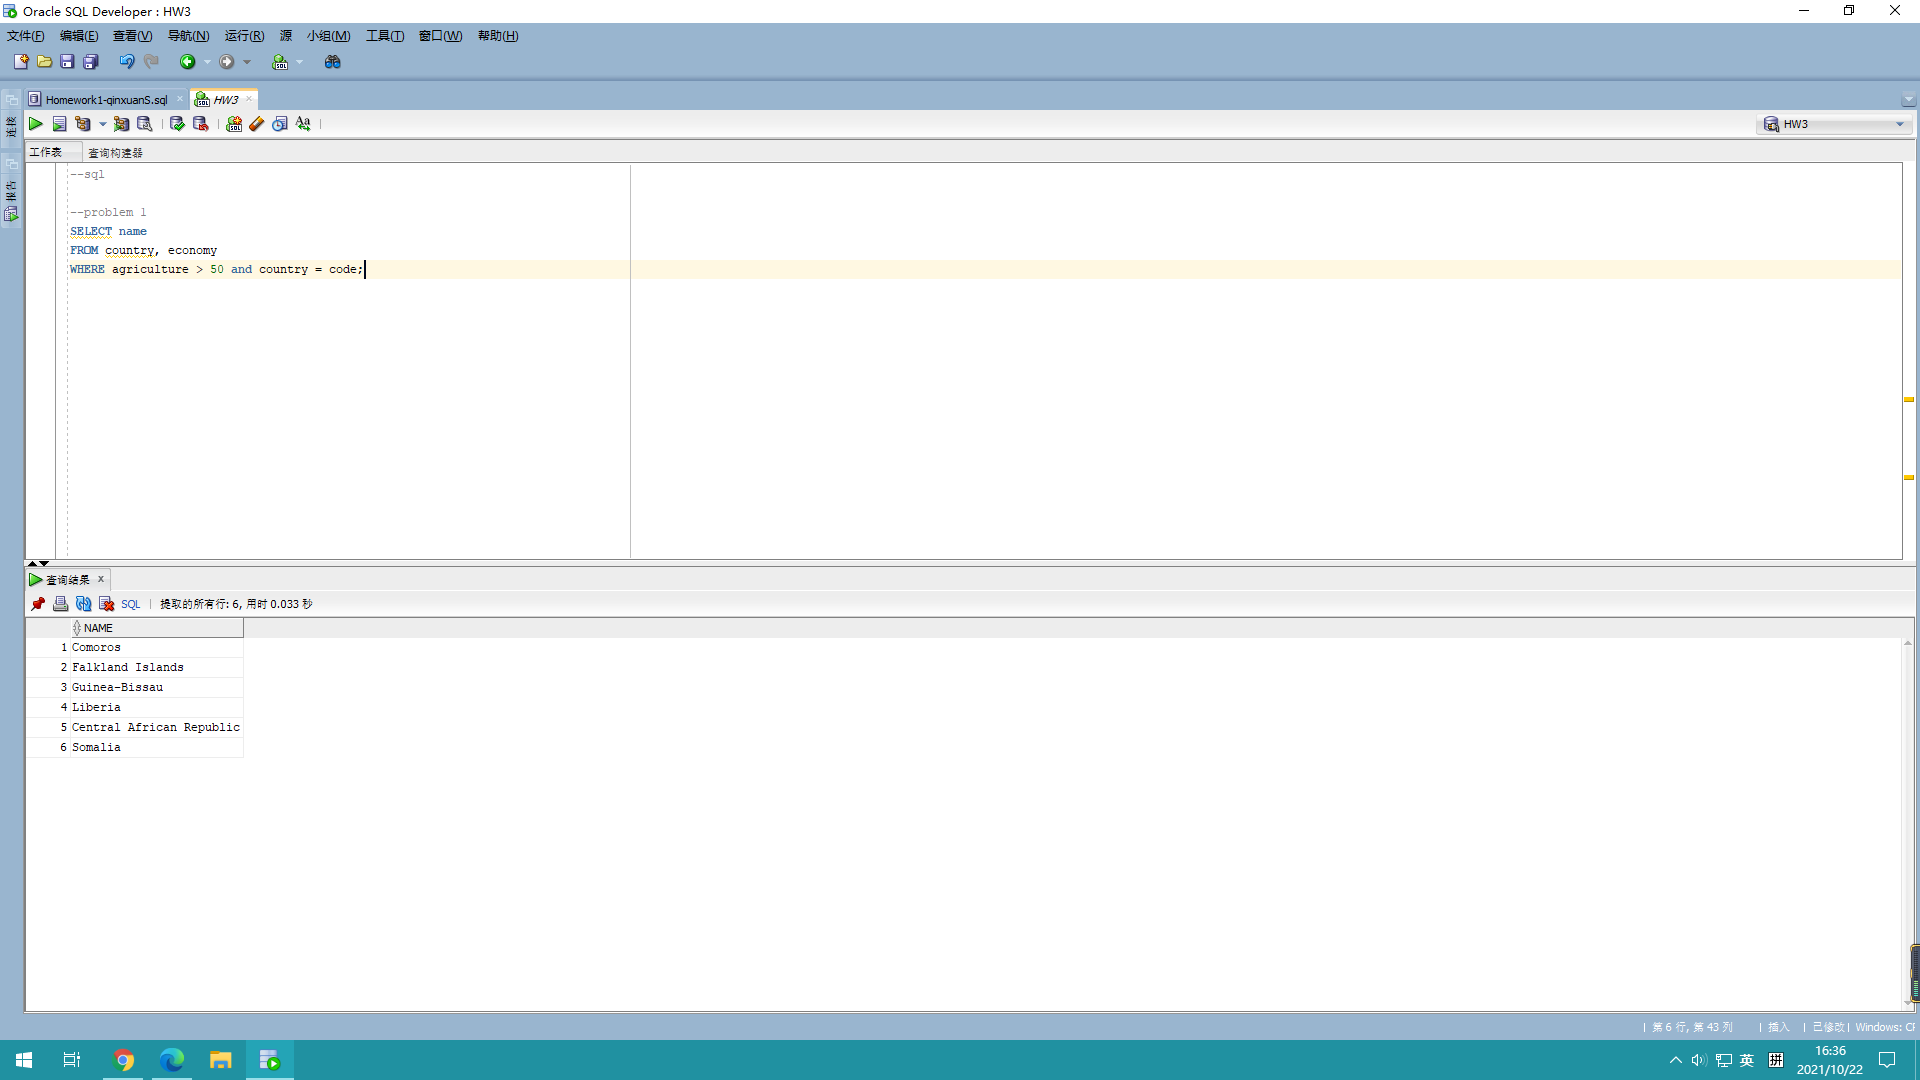
\includegraphics[width=1\linewidth]{../screen/p1}
		\caption{p1}
		\label{fig:p1}
	\end{figure}
	
	\noindent 2. [3 points] List the top five countries that will have the largest population after five years. [Assume that the population in five years is equal to the population this year * $(1 + growth rate)^{5}$. The population growth in the database schema is in percentage and should be divided by 100. Use the new attributes Country, Population after 5 years, and Rank for the resulting table schema.   \\
	
	\begin{lstlisting}[language=] 
SELECT Country, Population_after_5_years, rank() OVER (ORDER BY Population_after_5_years DESC) as Rank
FROM (SELECT name as Country, population*POWER(1+population_growth/100, 5)
 	as Population_after_5_years
	FROM country, population
	WHERE country = code
	ORDER BY Population_after_5_years DESC)
WHERE Population_after_5_years is NOT NULL and ROWNUM <=5;
	\end{lstlisting} 
	Output screen snapshots:
	\begin{figure}[H]
		\centering
		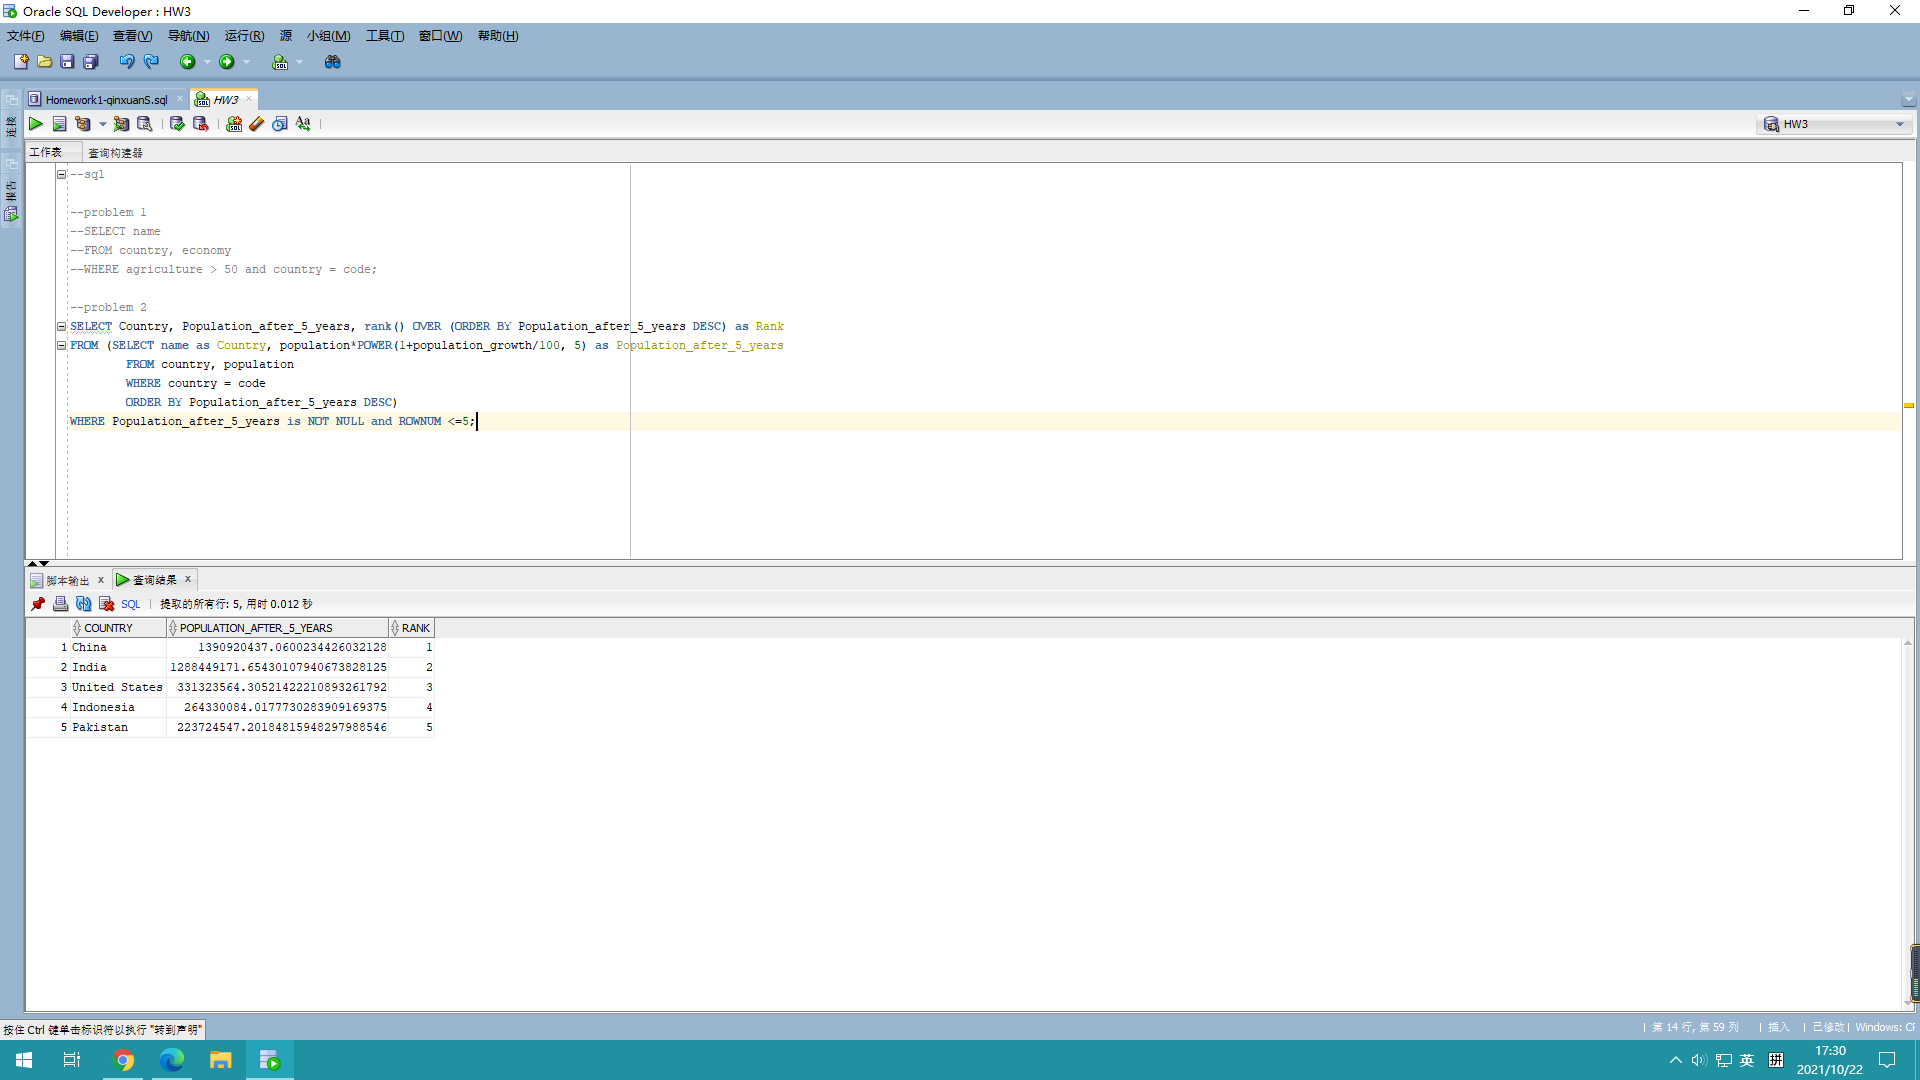
\includegraphics[width=1\linewidth]{../screen/p2}
		\caption{p2}
		\label{fig:p2}
	\end{figure}
	
	\noindent 3. [4 points] Find the country c1 that used to have the maximum number n1 of countries/areas depending on it. Further, find the country c2 that now has the maximum number n2 of countries/areas depending on it. Output c1, n1, c2, n2, and the difference between n1 and n2.   \\
	
	\begin{lstlisting}[language=] 
with WASD(wasdependent, numWD) as
  (SELECT wasdependent, COUNT(*) as numWD FROM politics WHERE wasdependent is not null 
	GROUP BY wasdependent)
SELECT wasdependent as c1, numWD as n1, dependent as c2, numD as n2, (numWD-numD) as difference
FROM WASD,
	(SELECT dependent, COUNT(*) as numD FROM politics WHERE dependent is not null 
	GROUP BY dependent)
WHERE numwd >= all(SELECT numwd from wasd) 
and numD >= all(select numd from 
	(SELECT dependent, COUNT(*) as numD FROM politics 
	WHERE dependent is not null GROUP BY dependent)
);
	\end{lstlisting} 
	Output screen snapshots:
	\begin{figure}[H]
		\centering
		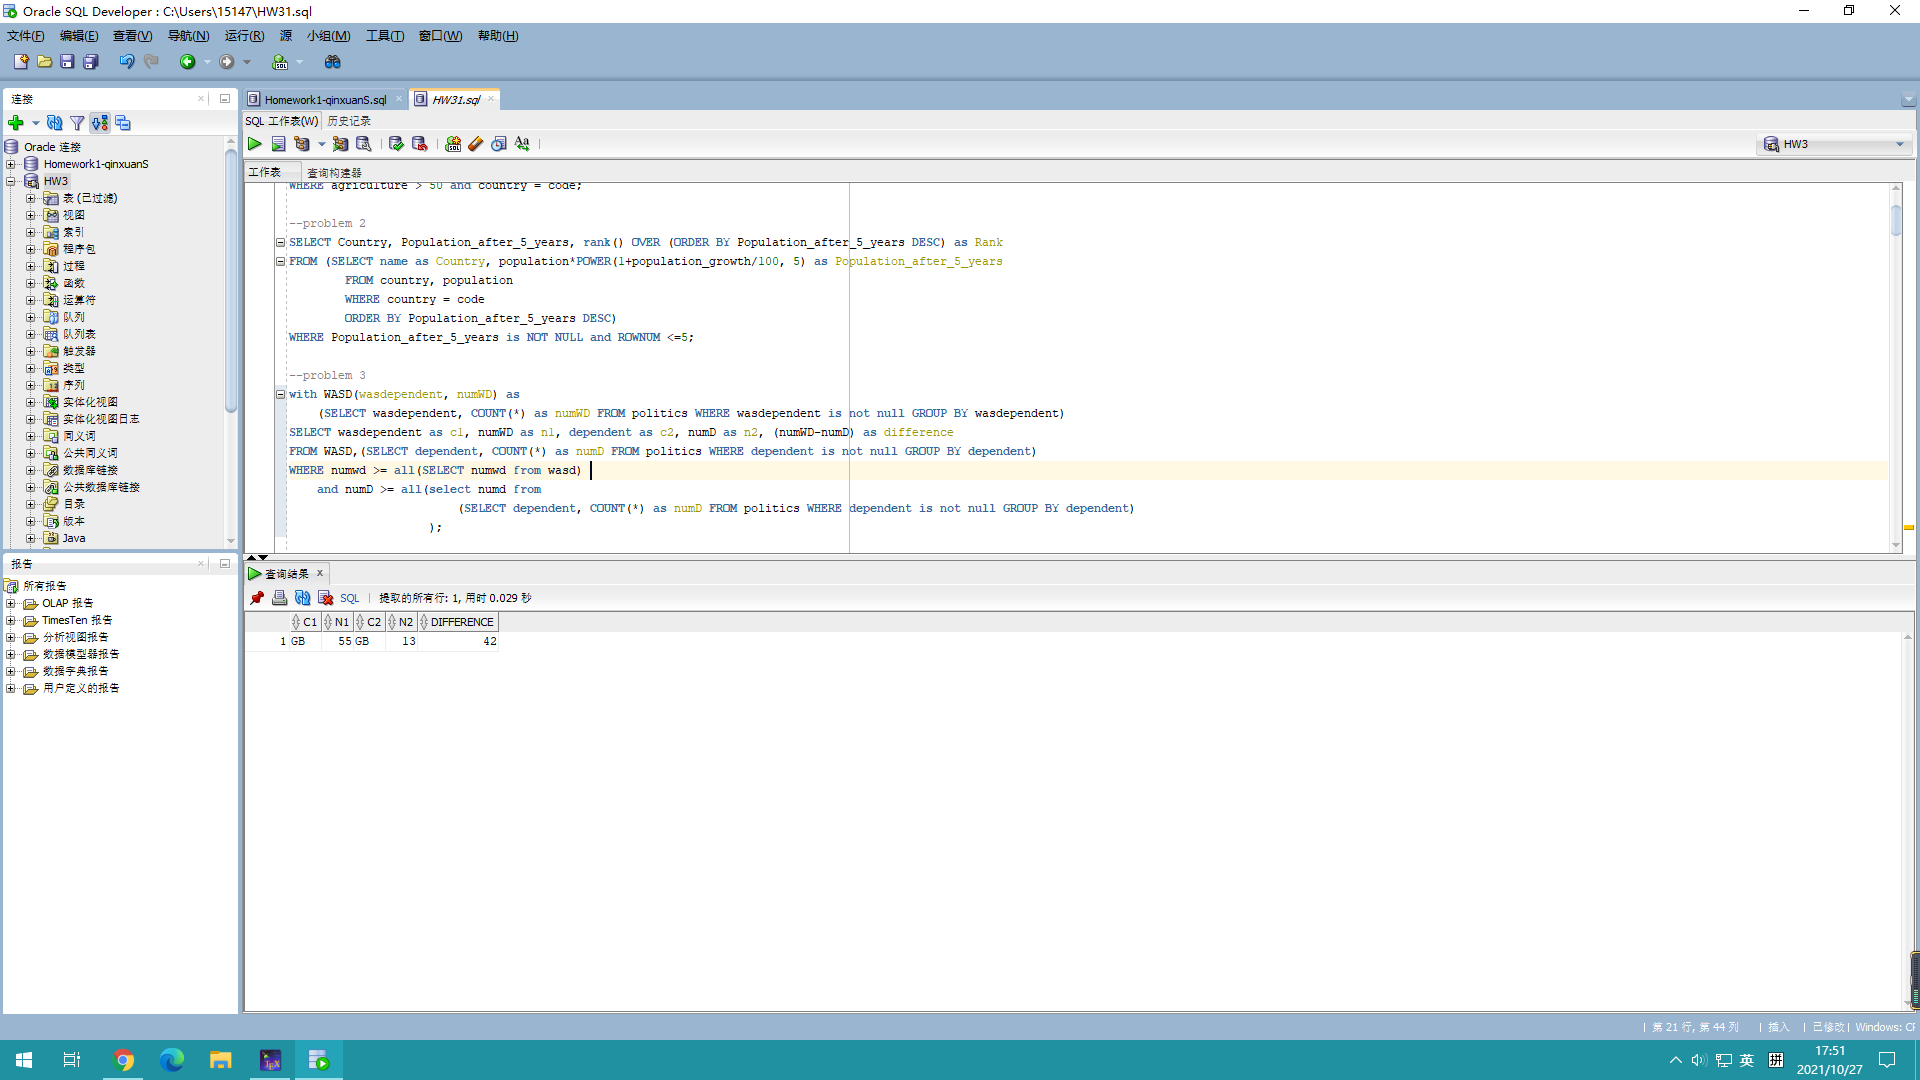
\includegraphics[width=1\linewidth]{../screen/p3}
		\caption{p3}
		\label{fig:p3}
	\end{figure}
	
	\noindent 4. [4 points] List the country names that have more than 4 different kinds of religion and at least one religion takes more than 80\%.  \\
	
	\begin{lstlisting}[language=] 
SELECT name
FROM country
WHERE code in (
SELECT country FROM religion GROUP BY country HAVING COUNT(name) >= 4 
	and MAX(percentage)>80);
	\end{lstlisting} 
	Output screen snapshots:
	\begin{figure}[H]
		\centering
		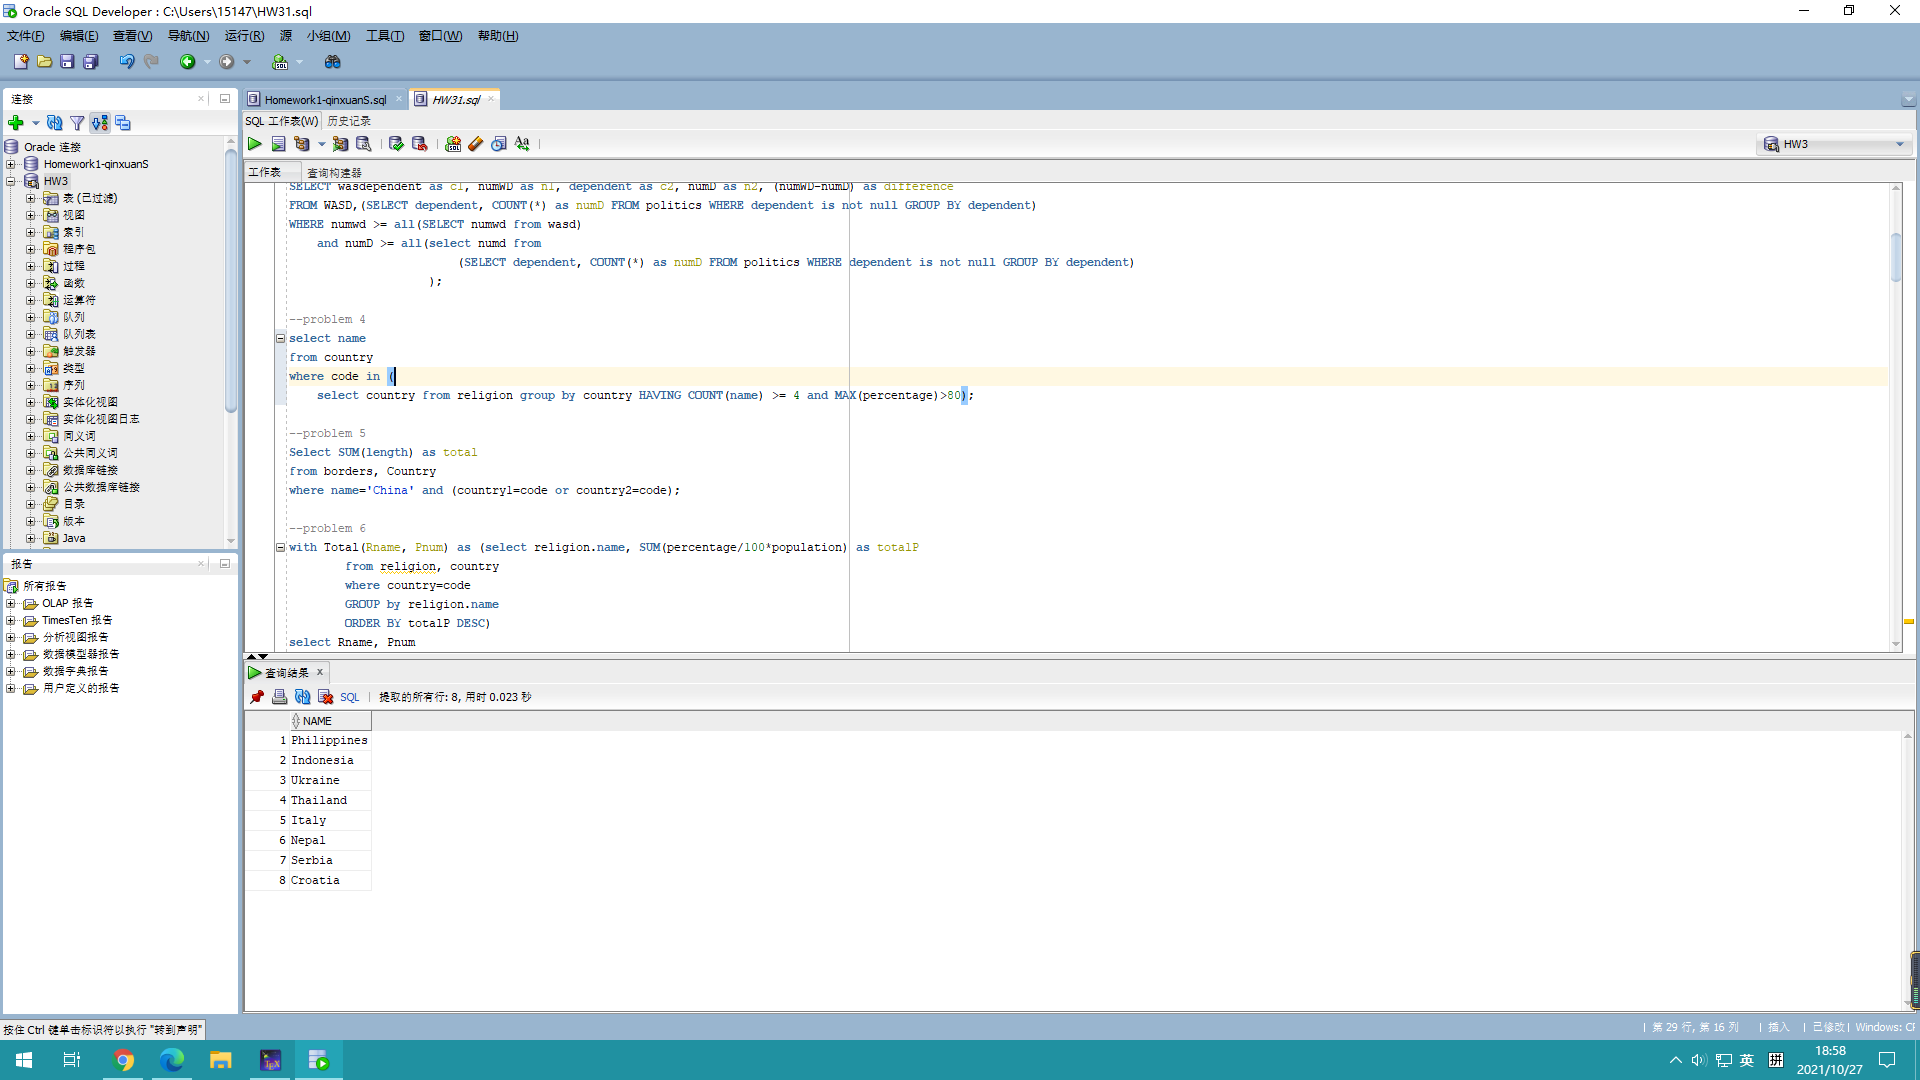
\includegraphics[width=0.8\linewidth]{../screen/p4}
		\caption{p4}
		\label{fig:p4}
	\end{figure}
	
	\noindent 5. [3 points] Compute the total length of the border that China shares with its neighboring countries.  \\
	
	\begin{lstlisting}[language=] 
SELECT SUM(length) as total
FROM borders, Country
WHERE name='China' and (country1=code or country2=code);
	\end{lstlisting} 
	Output screen snapshots:
	\begin{figure}[H]
		\centering
		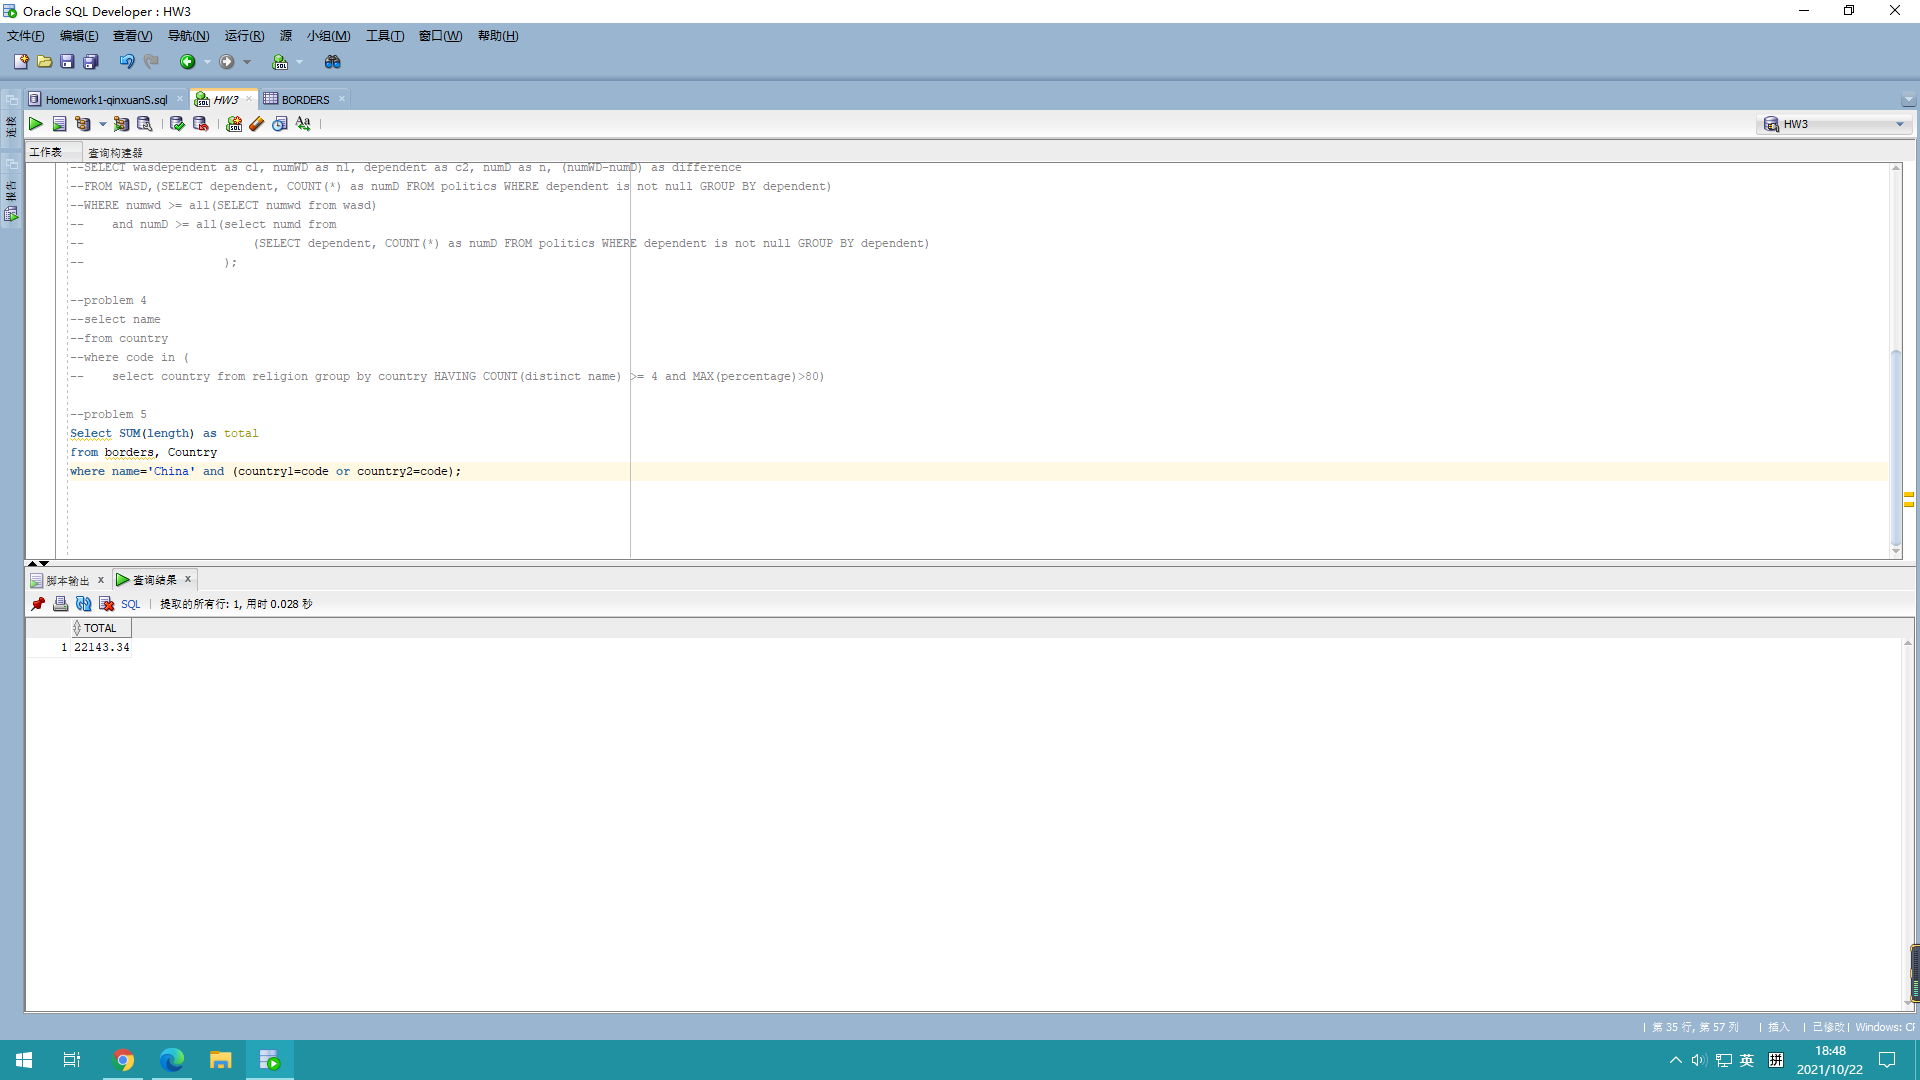
\includegraphics[width=1\linewidth]{../screen/p5}
		\caption{p5}
		\label{fig:p5}
	\end{figure}
	
	\noindent 6. [4 points] Find the top five popular religions and the numbers of their believers in the world.  \\
	
	\begin{lstlisting}[language=] 
with Total(Rname, Pnum) as 
(SELECT religion.name, SUM(percentage/100*population) as totalP
	FROM religion, country
	WHERE country=code
	GROUP by religion.name
	ORDER BY totalP DESC)
SELECT Rname, Pnum
FROM Total
WHERE ROWNUM <=5;
	\end{lstlisting} 
	Output screen snapshots:
	\begin{figure}[H]
		\centering
		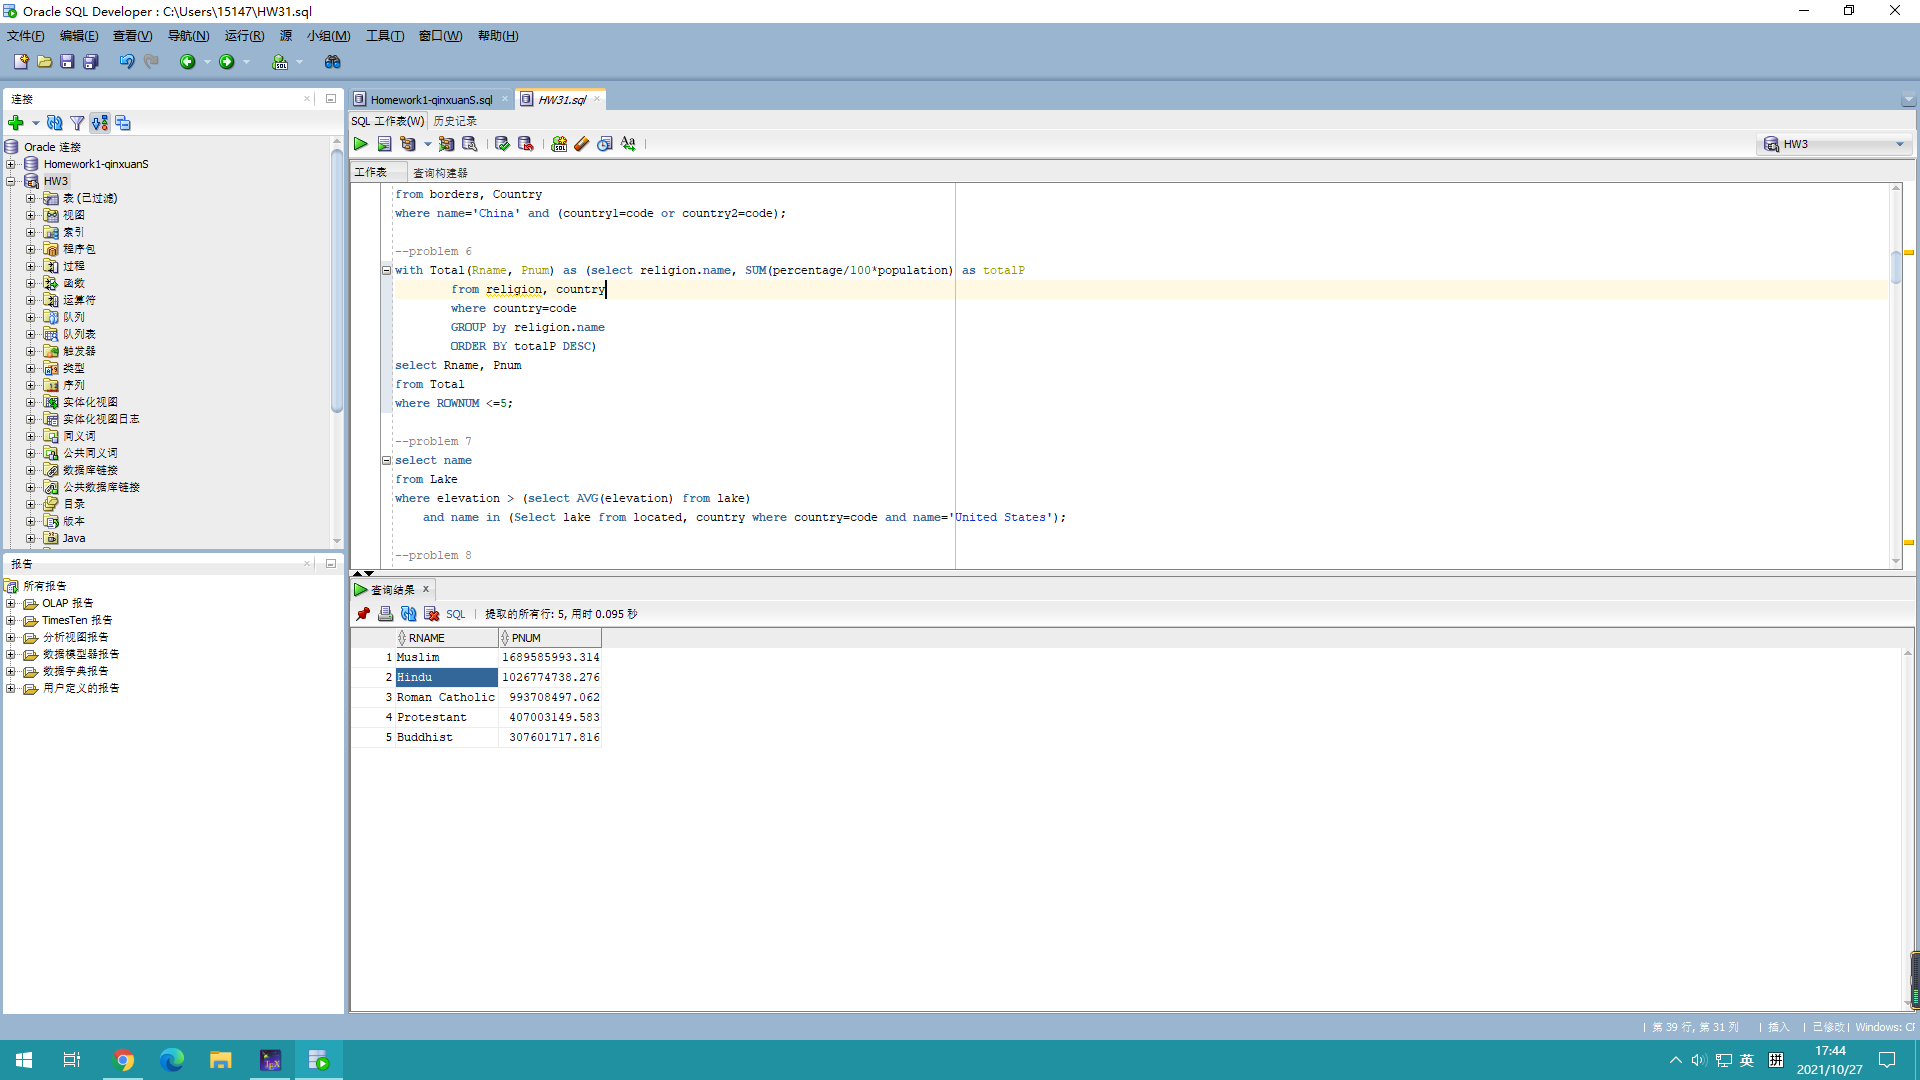
\includegraphics[width=0.9\linewidth]{../screen/p6}
		\caption{p6}
		\label{fig:p6}
	\end{figure}
	
	\noindent 7. [3 points] Find the names of the lakes in the United States with an elevation that is above the average elevation of all lakes world-wide.\\
	
	\begin{lstlisting}[language=] 
SELECT name
FROM Lake
WHERE elevation > (SELECT AVG(elevation) FROM lake) 
  and name in (SELECT lake FROM located, country where country=code and name='United States');
	\end{lstlisting} 
	Output screen snapshots:
	\begin{figure}[H]
		\centering
		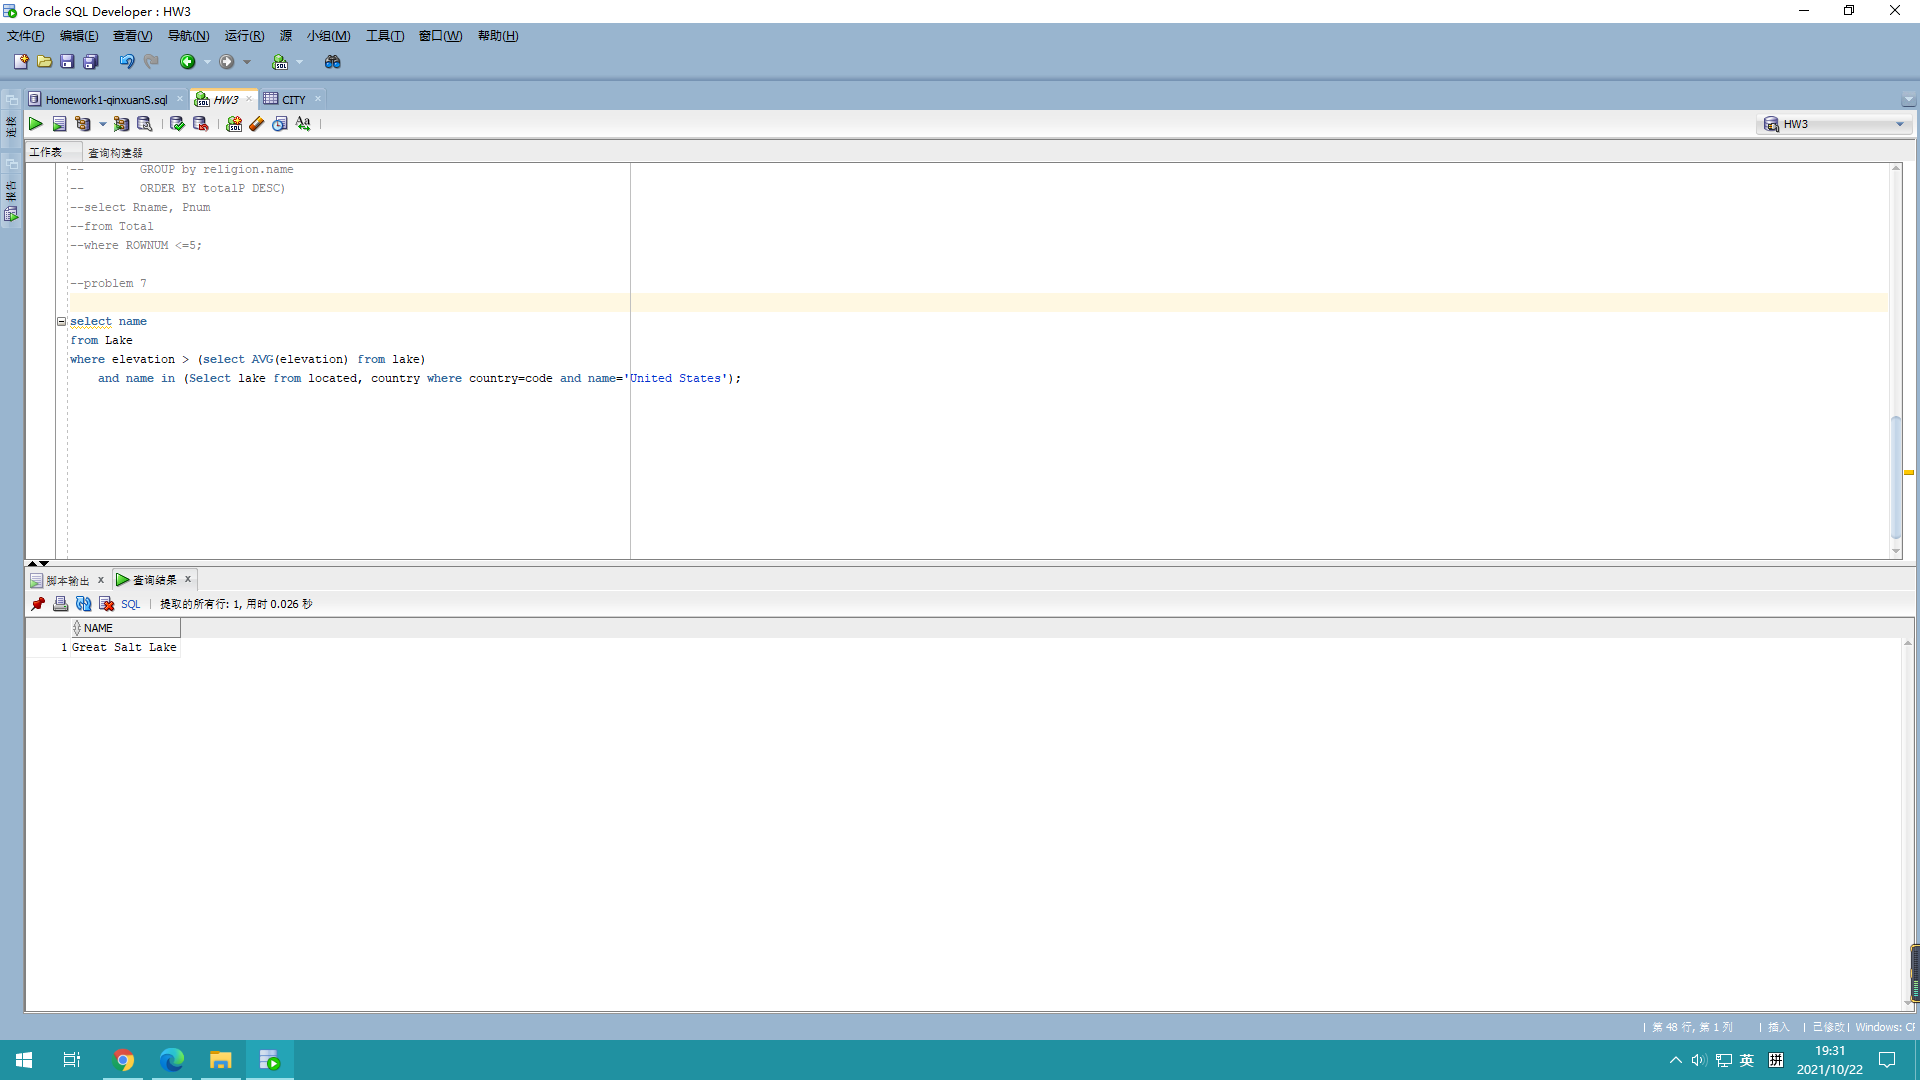
\includegraphics[width=0.9\linewidth]{../screen/p7}
		\caption{p7}
		\label{fig:p7}
	\end{figure}
	
	\noindent 8. [4 points] Find the largest population density (population/area) of provinces that have mountains of the “volcano” type. Output the province name, mountain name, and the population density.  \\
	
	\begin{lstlisting}[language=] 
SELECT name, mountain, density 
FROM (SELECT name, mountain, (population/area) as density
	FROM province, geo_mountain
	WHERE name=province and mountain in (SELECT name FROM mountain WHERE type='volcano')
	ORDER BY density DESC)
WHERE  ROWNUM <=1 ; 
	\end{lstlisting} 
	Output screen snapshots:
	\begin{figure}[H]
		\centering
		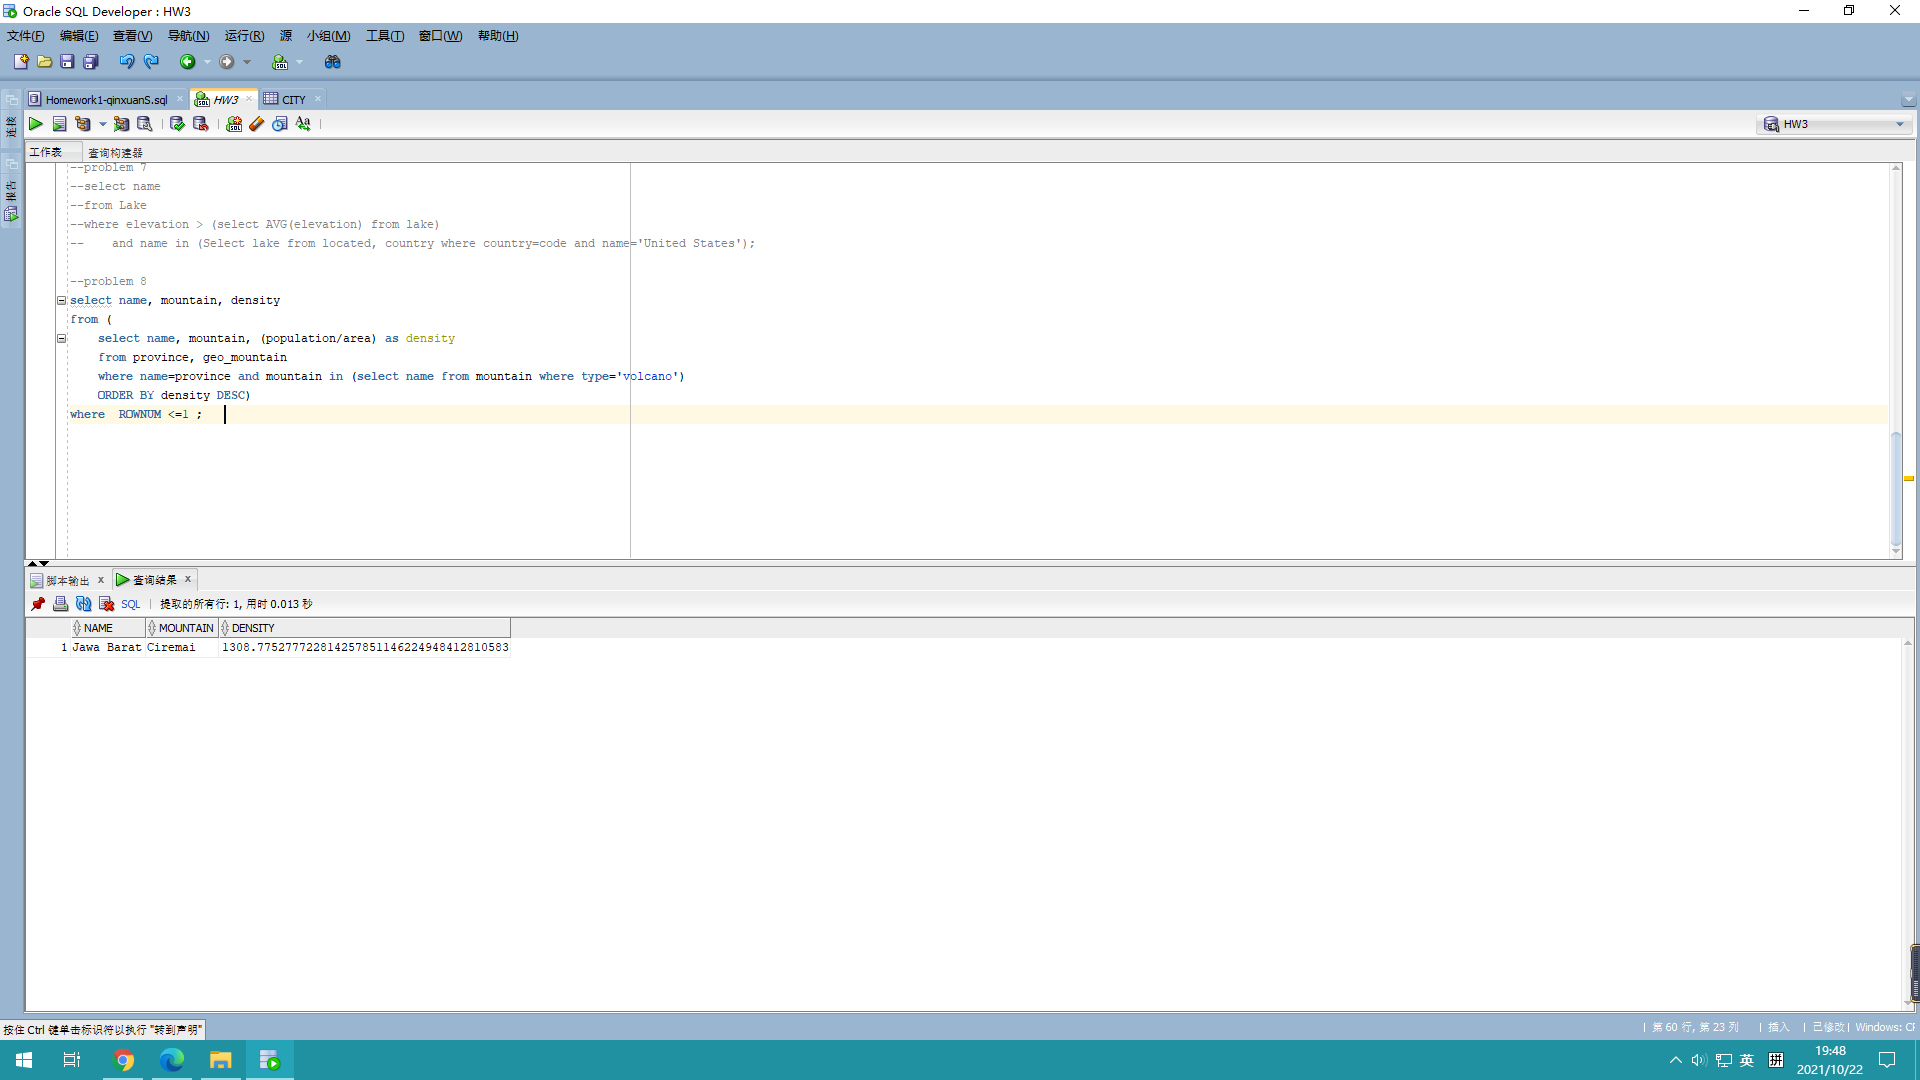
\includegraphics[width=1\linewidth]{../screen/p8}
		\caption{p8}
		\label{fig:p8}
	\end{figure}
	
	\noindent 9. [3 points] Find the provinces that are located on more than 2 islands and whose country’s GDP is greater than 1000000.   \\
	
	\begin{lstlisting}[language=] 
SELECT locate
FROM (SELECT province as locate, COUNT(island) as numI
	  FROM locatedon
	  group by province), economy,province
WHERE locate=province.name and province.country=economy.country and economy.gdp>1000000 
	and numI>2;
	\end{lstlisting} 
	Output screen snapshots:
	\begin{figure}[H]
		\centering
		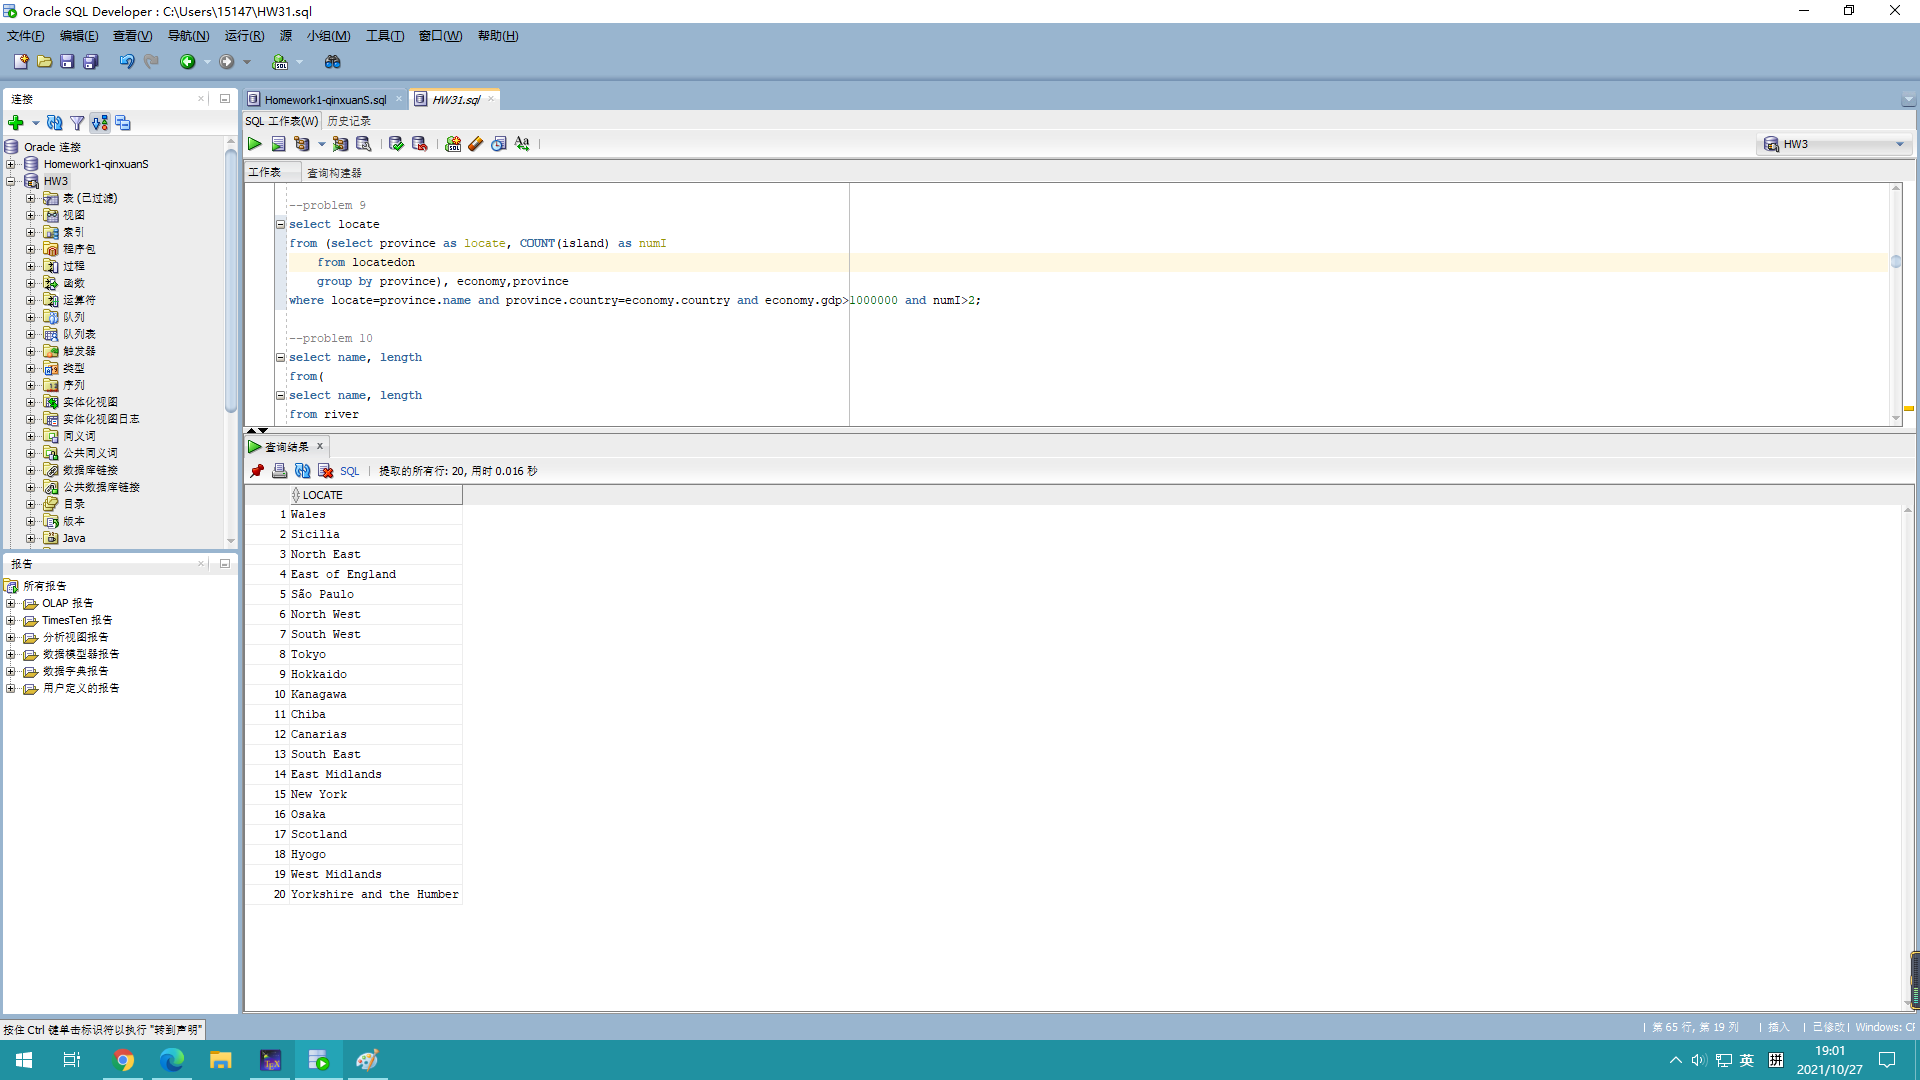
\includegraphics[width=0.8\linewidth]{../screen/p9}
		\caption{p9}
		\label{fig:p9}
	\end{figure}
	
	\noindent 10. [3 points] Find the two longest rivers that flow through at least one lake and that finally flow into the Atlantic Ocean. Output the name and the length of the rivers.  \\
	
	\begin{lstlisting}[language=] 
SELECT name, length
FROM(SELECT name, length
	FROM river
	WHERE sea='Atlantic Ocean' 
	  and name in (SELECT river as riverN
			FROM riverthrough
			GROUP BY river
			HAVING COUNT(lake) >= 1)
			ORDER BY length DESC
)
WHERE ROWNUM<=2;
	\end{lstlisting} 
	Output screen snapshots:
	\begin{figure}[H]
		\centering
		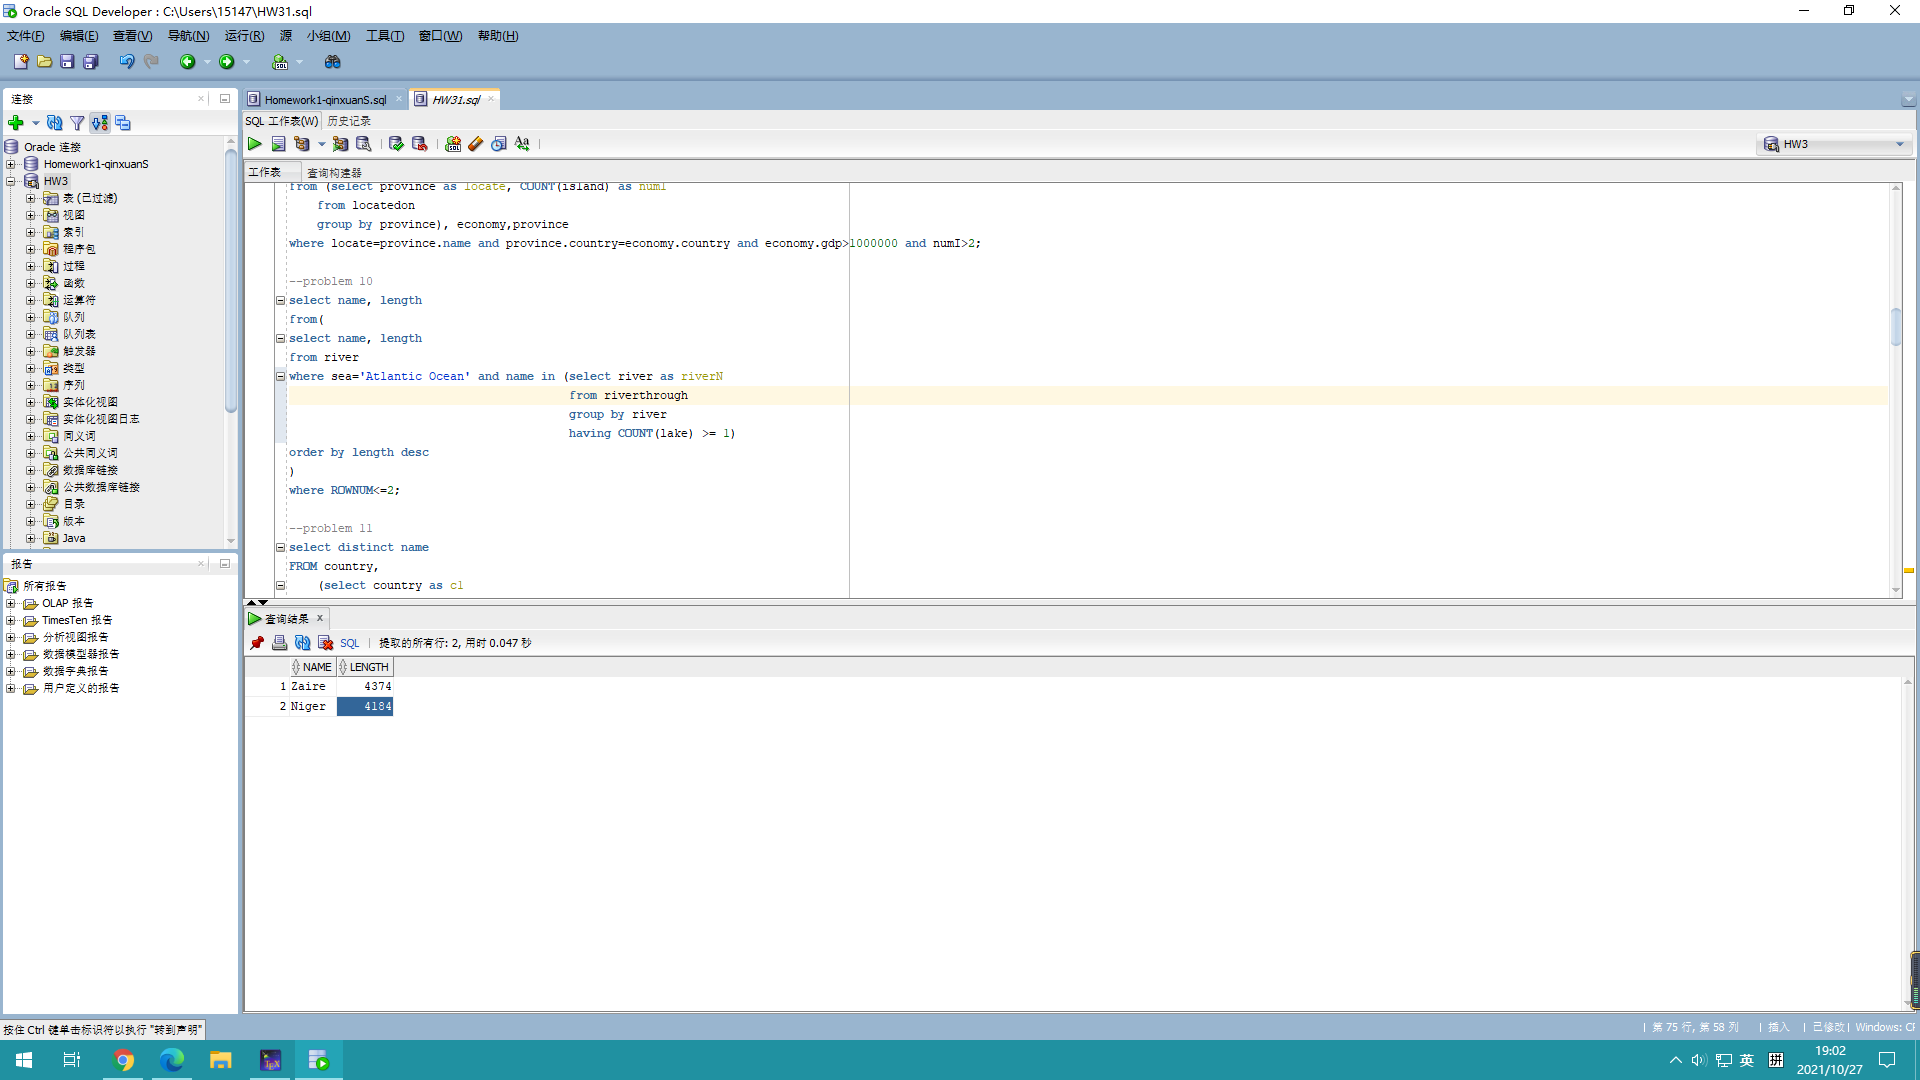
\includegraphics[width=0.75\linewidth]{../screen/p10}
		\caption{p10}
		\label{fig:p10}
	\end{figure}
	
	\noindent 11. [4 points] Determine the names of countries that have more than three rivers and that have lakes next to more than three provinces.  \\
	
	\begin{lstlisting}[language=] 
SELECT distinct name 
FROM country, 
  (SELECT country AS c1
	FROM located
	GROUP BY country
	HAVING COUNT(river)>3),
  (SELECT country AS c2
	FROM located 
	WHERE lake in ( select lake
			FROM located
			WHERE lake is not null
			GROUP BY lake
			HAVING COUNT(province)>3))
WHERE code=c1 and code = c2 and c1=c2;
	\end{lstlisting} 
	Output screen snapshots:
	\begin{figure}[H]
		\centering
		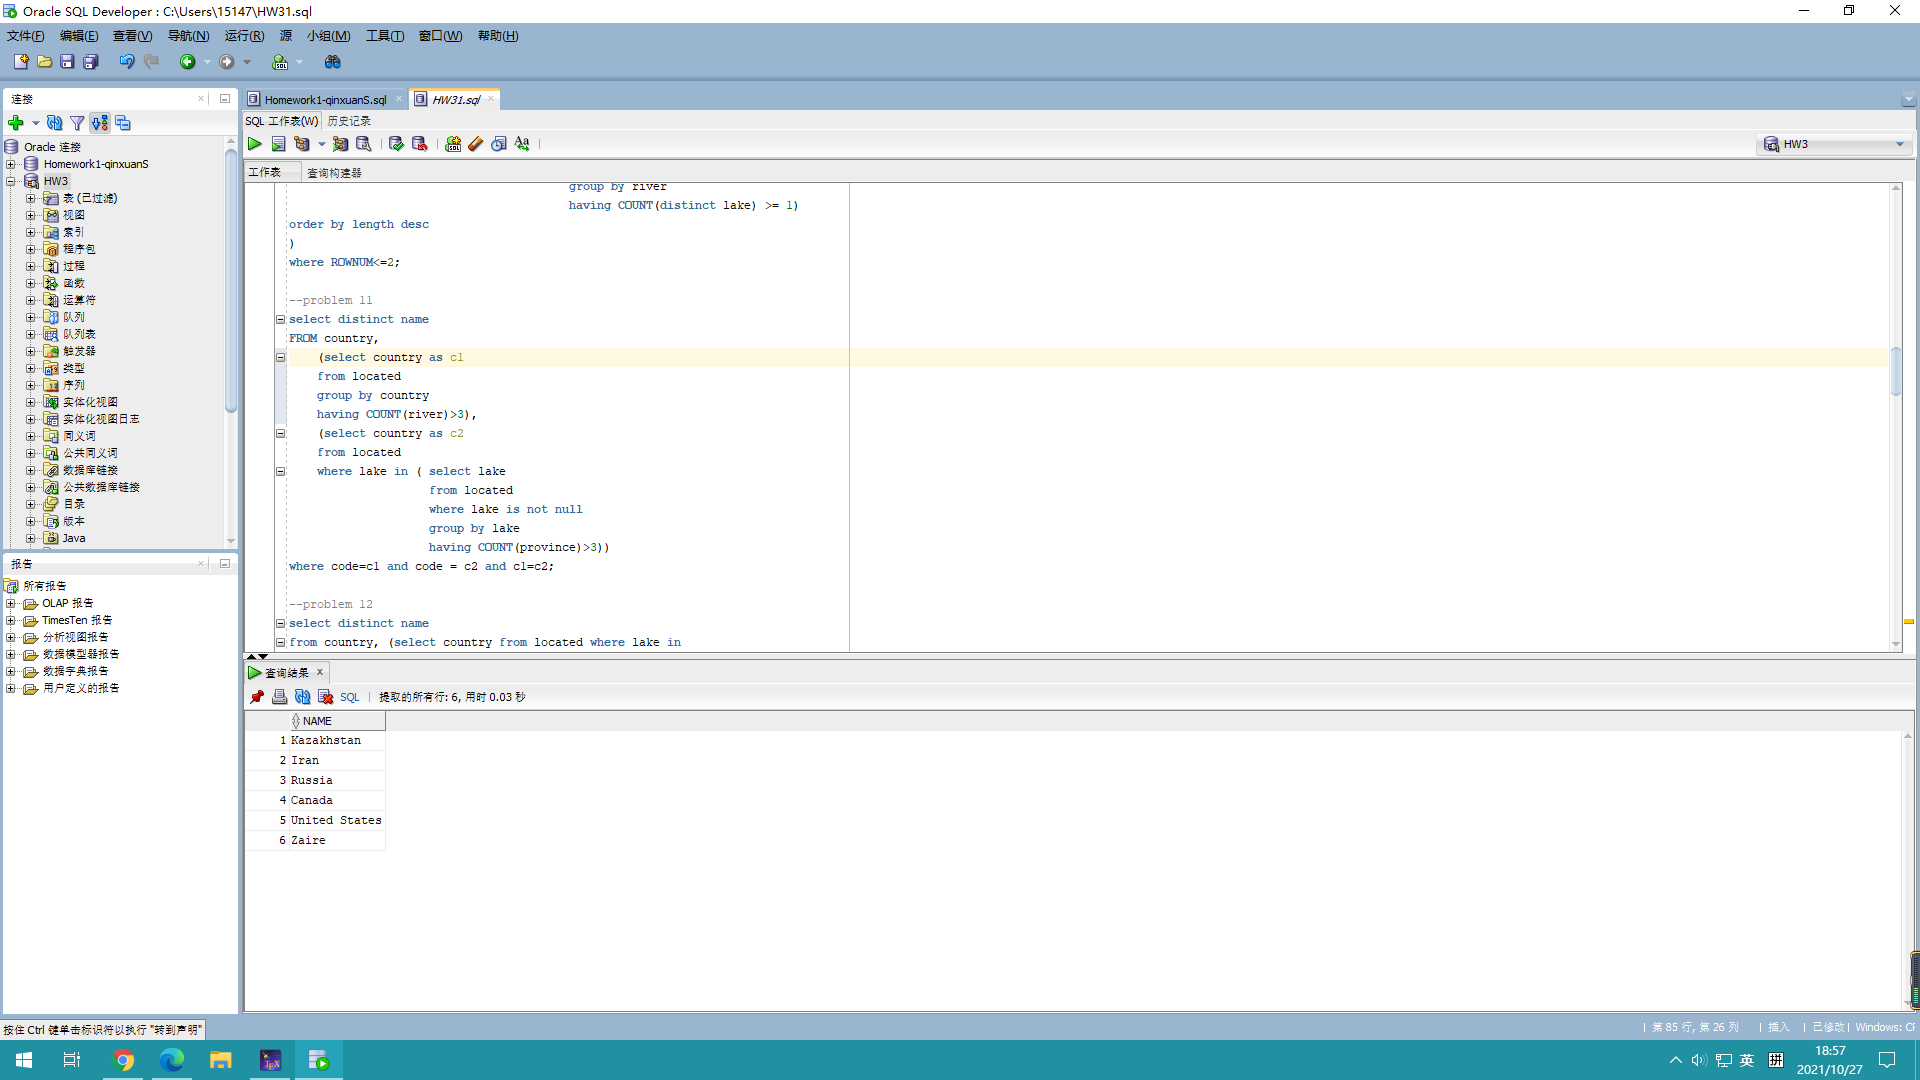
\includegraphics[width=1\linewidth]{../screen/p11}
		\caption{p11}
		\label{fig:p11}
	\end{figure}
	
	\noindent 12. [4 points] Find the names of those countries that are bounded by the largest lake.		\\
	
	\begin{lstlisting}[language=] 
SELECT distinct name
FROM country, (SELECT country FROM located WHERE lake in (
		SELECT name 
		FROOM lake
		WHERE area=(SELECT MAX(area) FROM lake))
		)
WHERE code=country;
	\end{lstlisting} 
	Output screen snapshots:
	\begin{figure}[H]
		\centering
		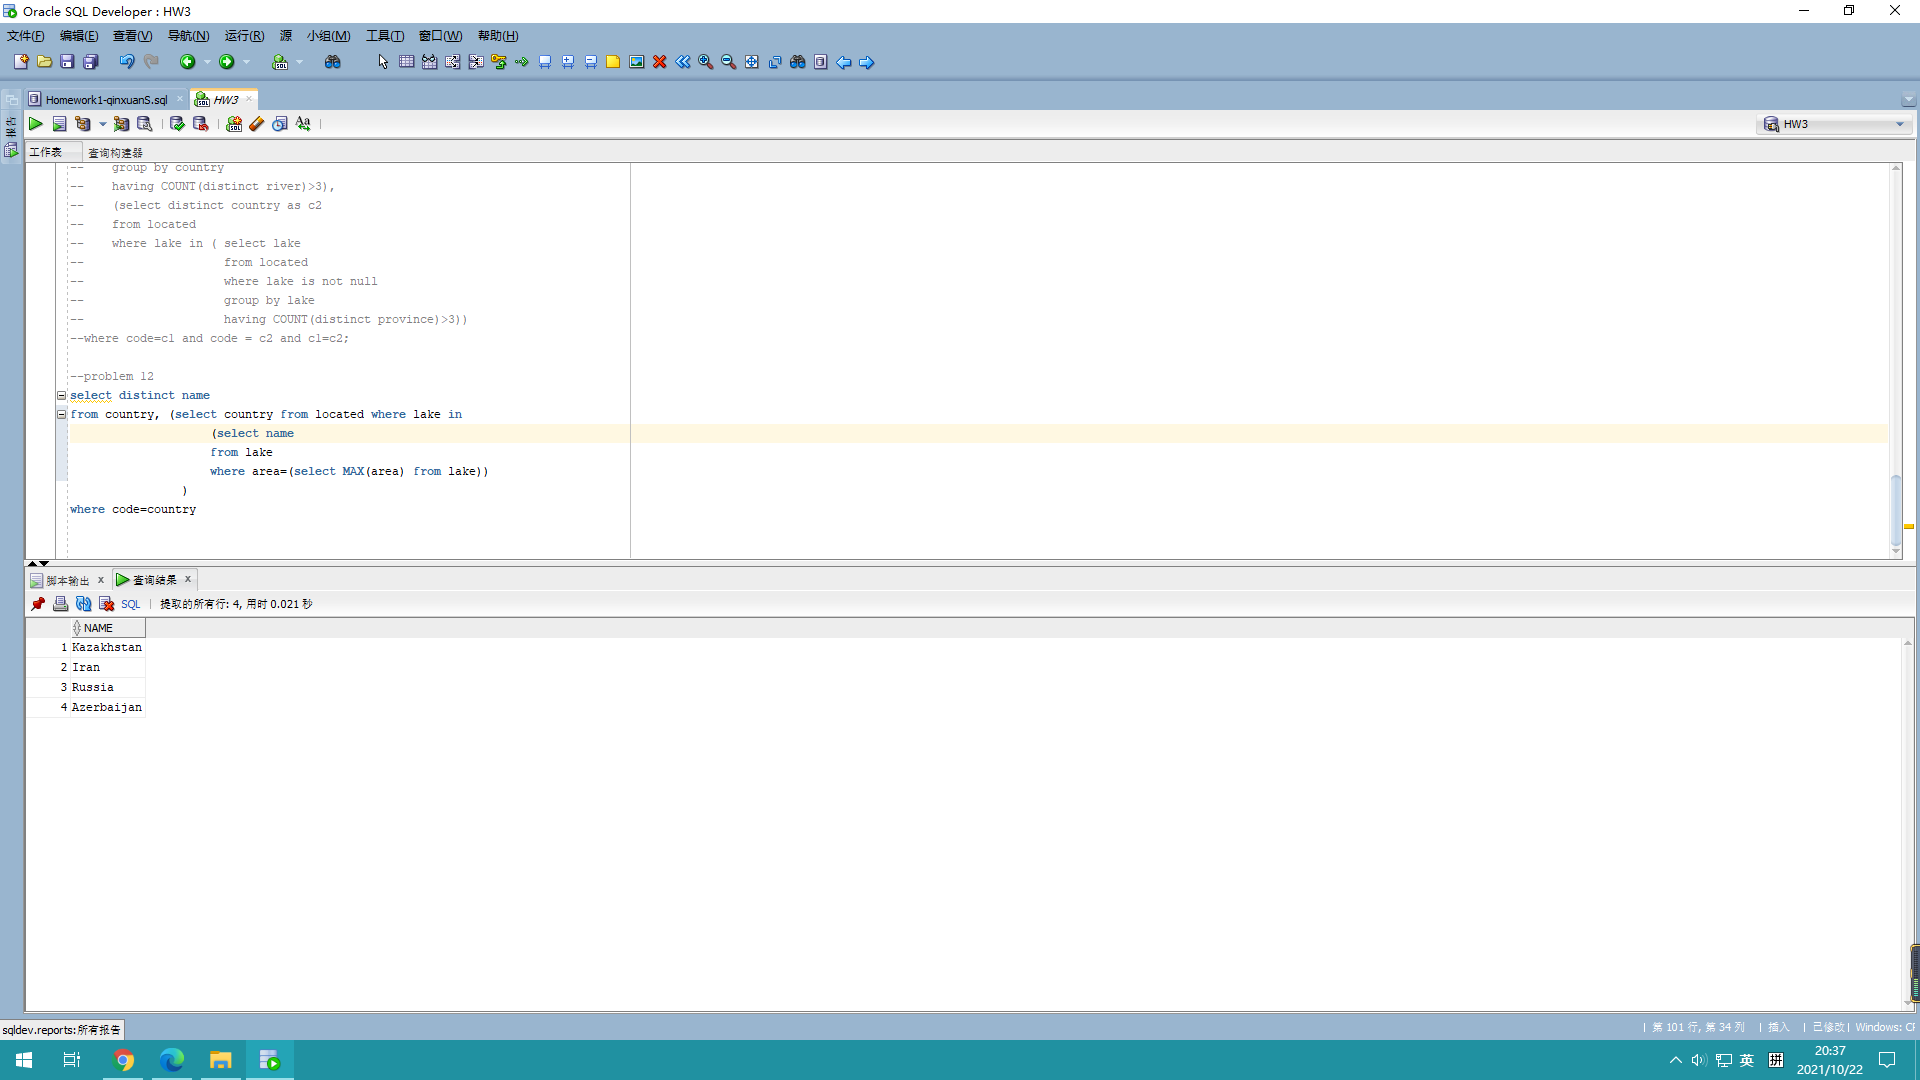
\includegraphics[width=0.85\linewidth]{../screen/p12}
		\caption{p12}
		\label{fig:p12}
	\end{figure}
	
	\noindent 13. [2 points] Find the height of the highest mountain for each continent.  \\
	
	\begin{lstlisting}[language=] 
with MountELe(continent, elevation) as 
(SELECT continent,elevation
	FROM geo_mountain, encompasses, mountain
	WHERE mountain=name and encompasses.country=geo_mountain.country
	GROUP BY continent, elevation)
SELECT continent, MAX(elevation)
FROM MountEle
GROUP BY continent;
	\end{lstlisting} 
	Output screen snapshots:
	\begin{figure}[H]
		\centering
		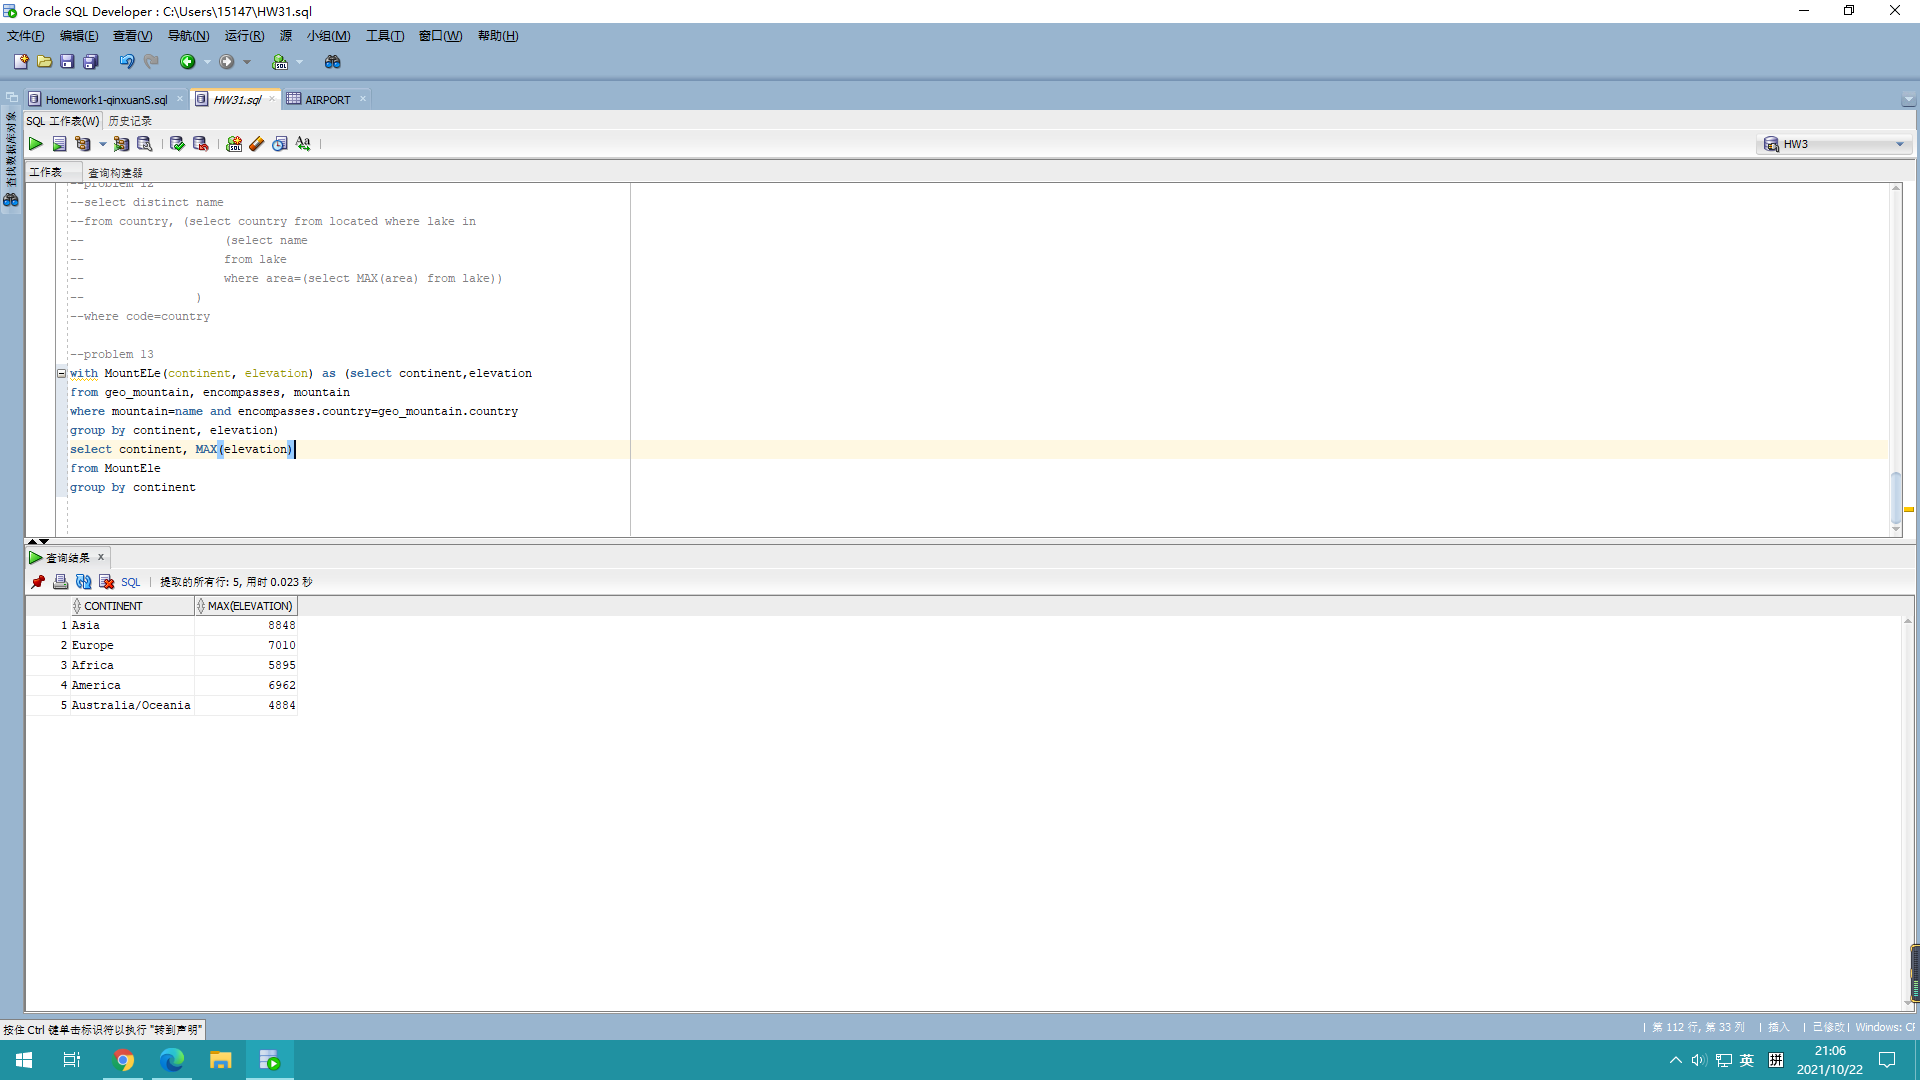
\includegraphics[width=0.85\linewidth]{../screen/p13}
		\caption{p13}
		\label{fig:p13}
	\end{figure}
	
	\noindent 14. [3 points] Find the countries whose depth of the deepest sea is less than the elevation of the highest mountain. Display the country name, depth of its deepest sea, and the elevation of the highest mountain. \\
	
	\begin{lstlisting}[language=] 
SELECT name, d as depth, e as elevation
FROM country,(SELECT country as c1, max(depth) as d
		FROM located, sea
		WHERE sea.name=sea
		GROUP BY country),
		(SELECT country as c2, MAX(elevation) as e
		FROM geo_mountain, mountain
		WHERE mountain=name
		GROUP BY country)
WHERE c1=c2 and code = c1 and code =c2 and d<e;
	\end{lstlisting} 
	Output screen snapshots:
	\begin{figure}[H]
		\centering
		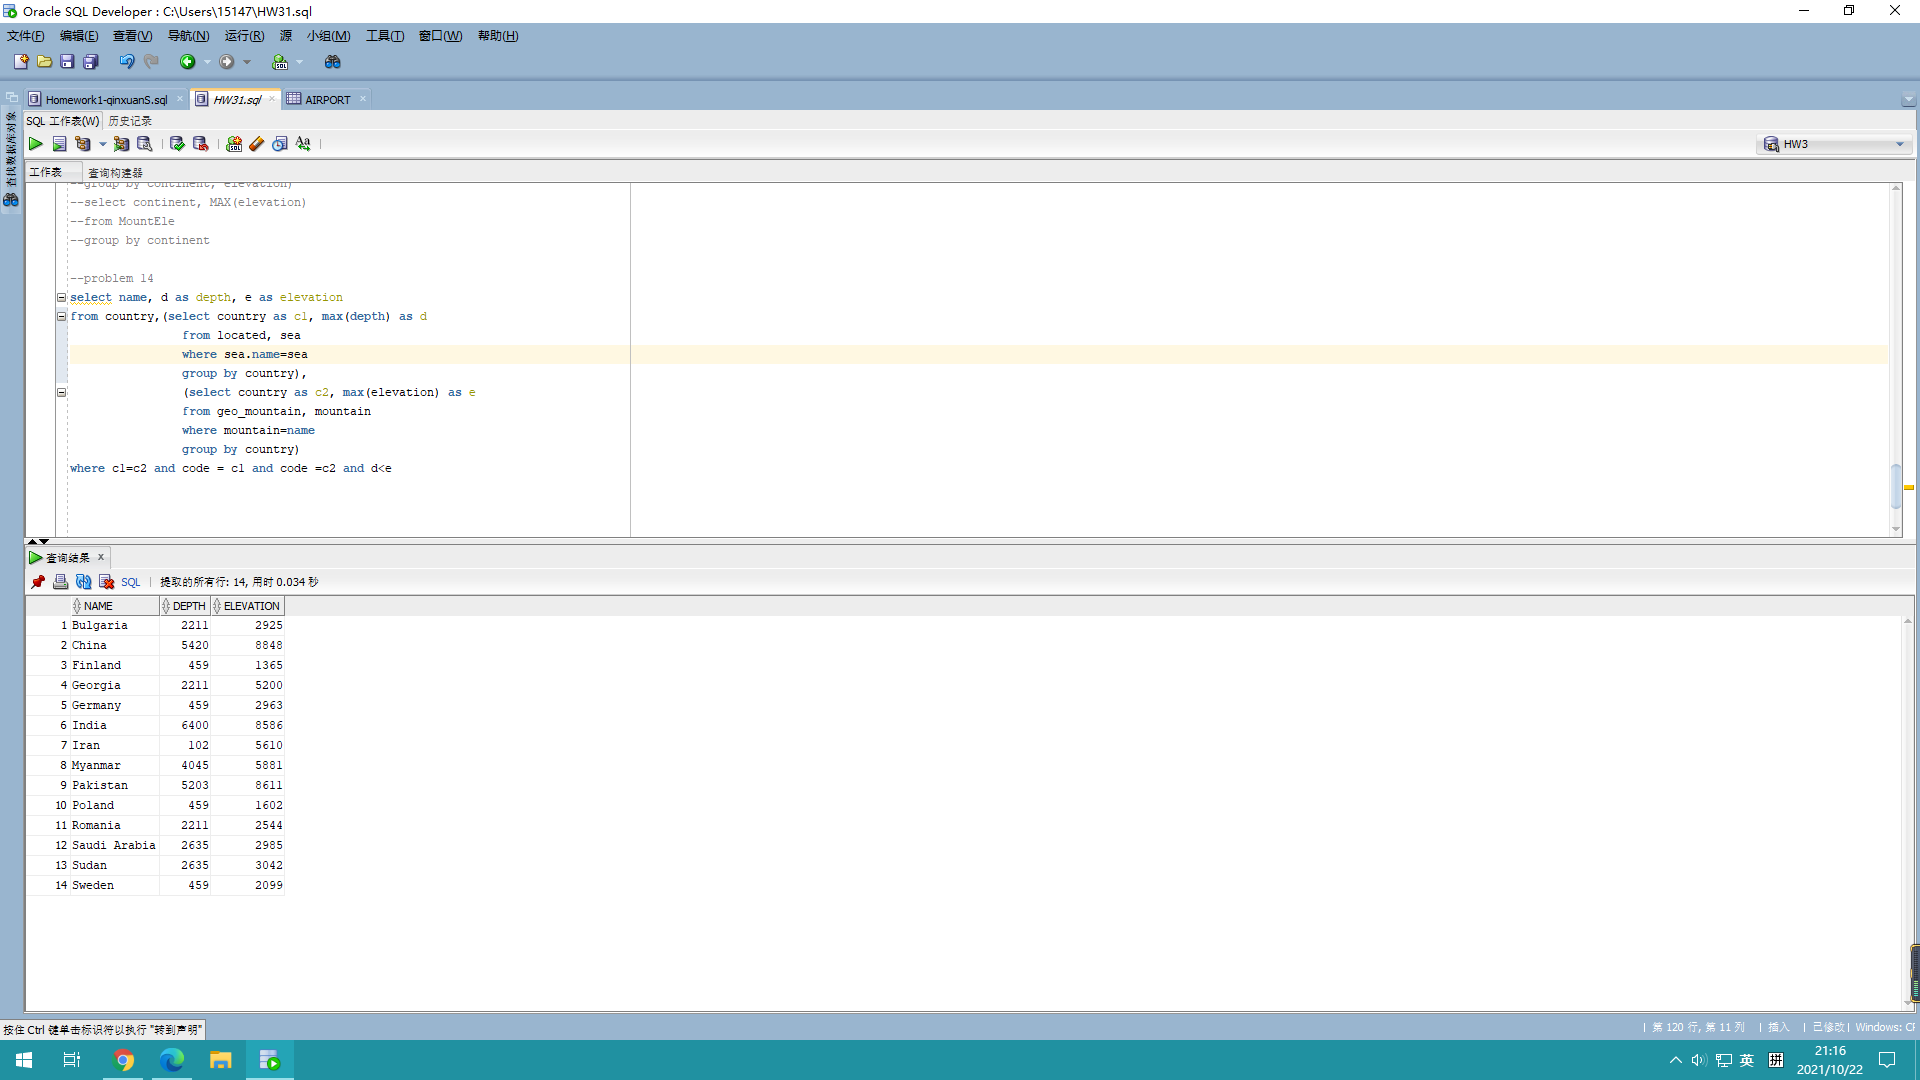
\includegraphics[width=1\linewidth]{../screen/p14}
		\caption{p14}
		\label{fig:p14}
	\end{figure}
	
	\noindent 15. [4 points] Find the northernmost cities of each continent (except Asia). Display the names of these cities and their continent. List cities that are northern of other cities in the result table first.   \\
	
	\begin{lstlisting}[language=] 
with cityCon(continent, maxL) as 
(SELECT continent, MAX(latitude)
	FROM city, encompasses
	WHERE encompasses.country = city.country
	GROUP BY continent)
SELECT continent, name
FROM cityCon, city
WHERE latitude in (maxL);
	\end{lstlisting} 
	Output screen snapshots:
	\begin{figure}[H]
		\centering
		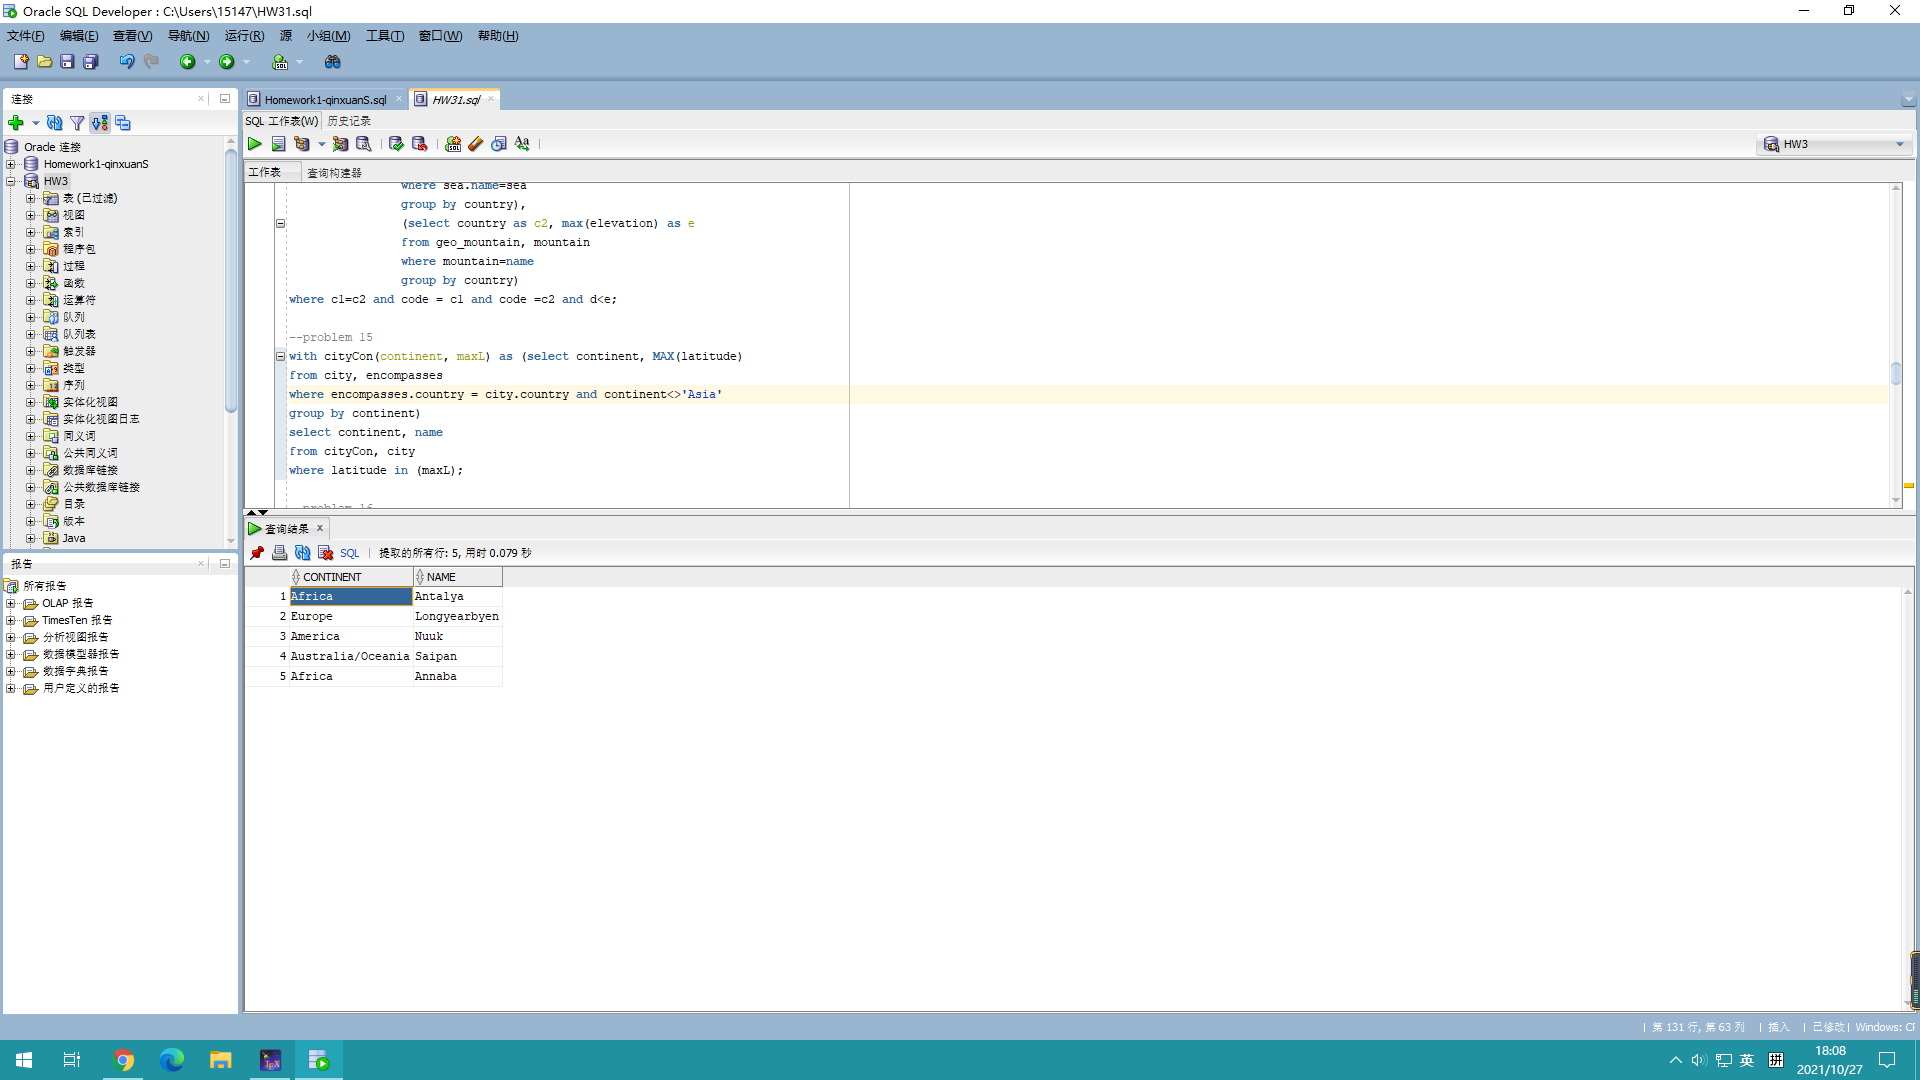
\includegraphics[width=0.92\linewidth]{../screen/p15}
		\caption{p15}
		\label{fig:p15}
	\end{figure}
	
	\noindent 16. [1 point] Find all countries whose capitals have positive latitudes and less than 10000 inhabitants.   \\
	
	\begin{lstlisting}[language=] 
SELECT name
FROM country
WHERE code in (SELECT country FROM city WHERE name = country.capital and 
	country=country.code and population<10000 and latitude>0);
	\end{lstlisting} 
	Output screen snapshots:
	\begin{figure}[H]
		\centering
		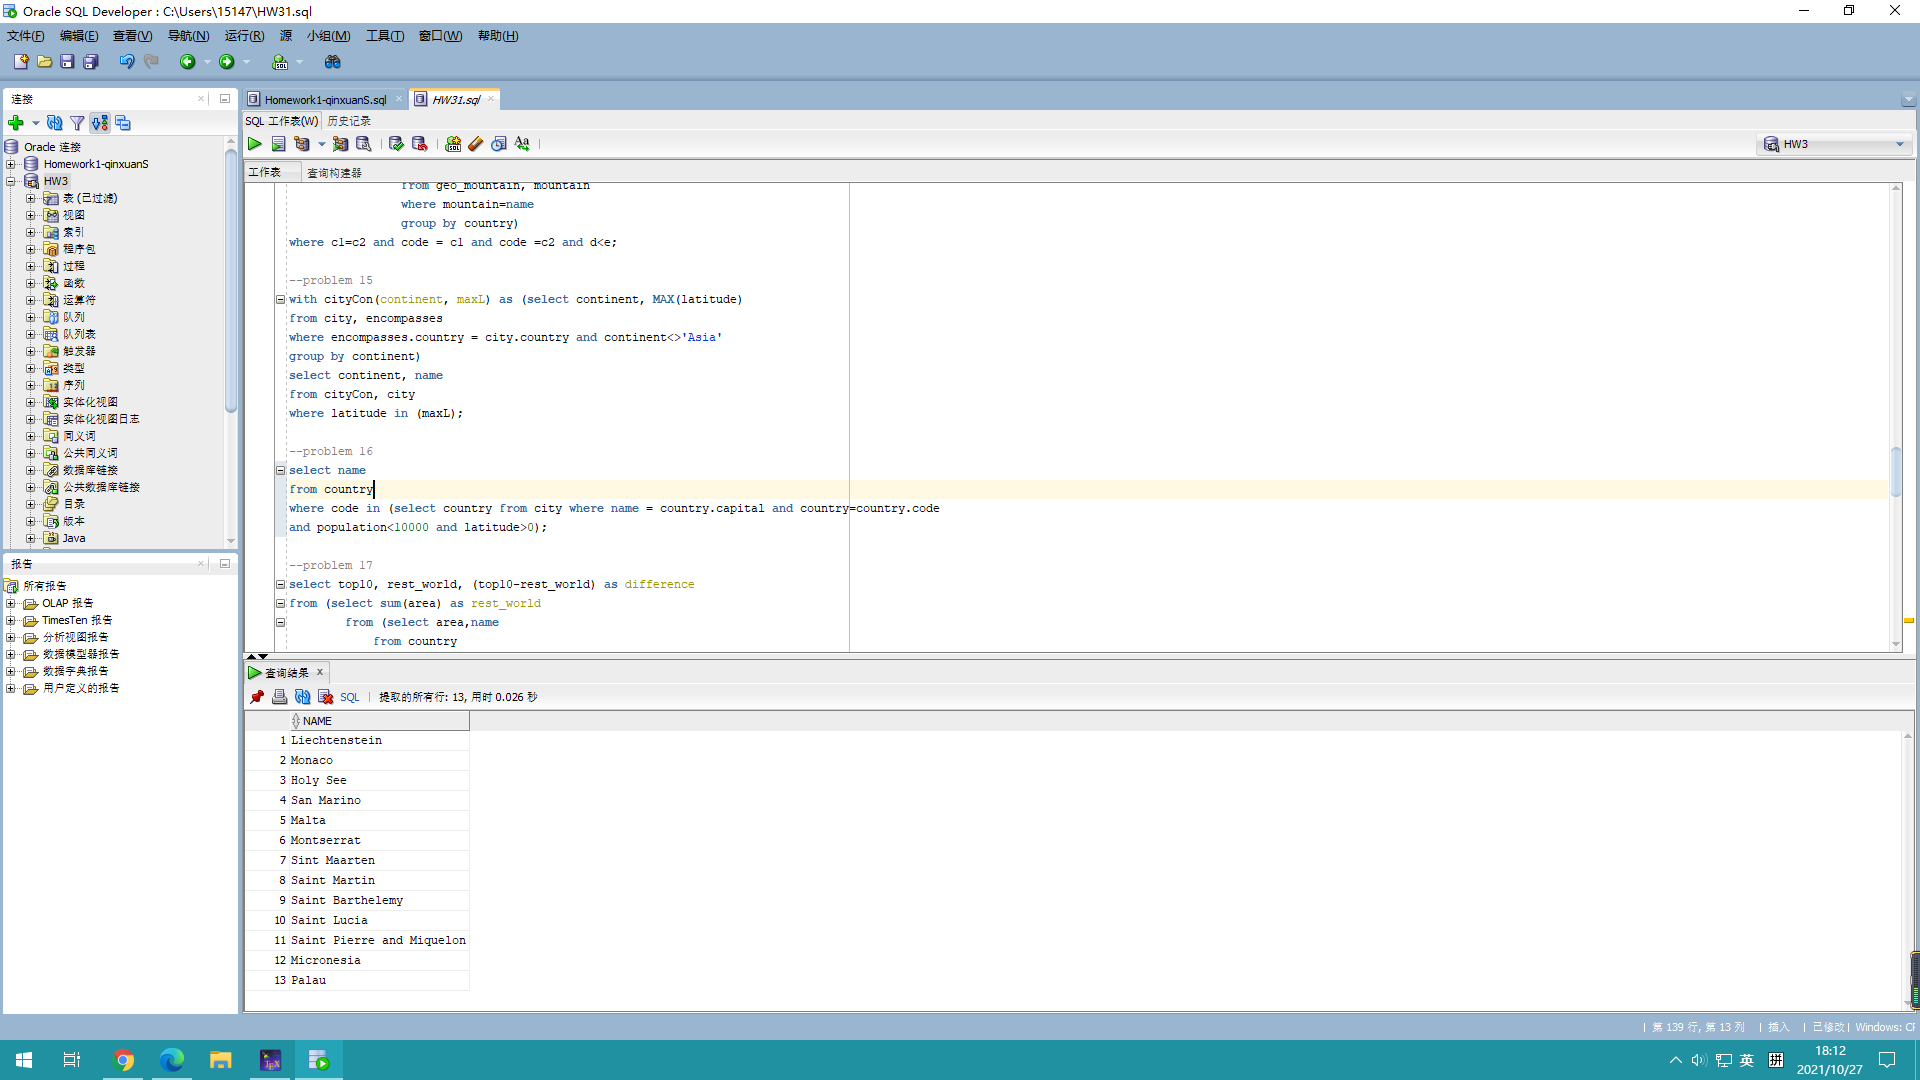
\includegraphics[width=0.95\linewidth]{../screen/p16}
		\caption{p16}
		\label{fig:p16}
	\end{figure}
	
	\noindent 17. [4 points] Find what is larger. Is it the sum of the areas of the 10 largest countries (attribute top10) or the sum of the areas of the remaining countries (attribute rest\_world)? What is their difference (attribute difference)? Display the values for the attributes top10, rest\_world, and difference.    \\
	
	\begin{lstlisting}[language=] 
SELECT top10, rest_world, (top10-rest_world) as difference
FROM (SELECT sum(area) as rest_world
	FROM (SELECT area,name 
		FROM country
		WHERE area is not null
		ORDER BY area), 
	    (SELECT COUNT(name) as numC FROM country)
        WHERE ROWNUM <= numC-10),
(SELECT sum(area) as top10
  FROM (SELECT area,name 
	FROM country
	WHERE area is not null
	ORDER BY area DESC)
  WHERE ROWNUM <= 10);
	\end{lstlisting} 
	Output screen snapshots:
	\begin{figure}[H]
		\centering
		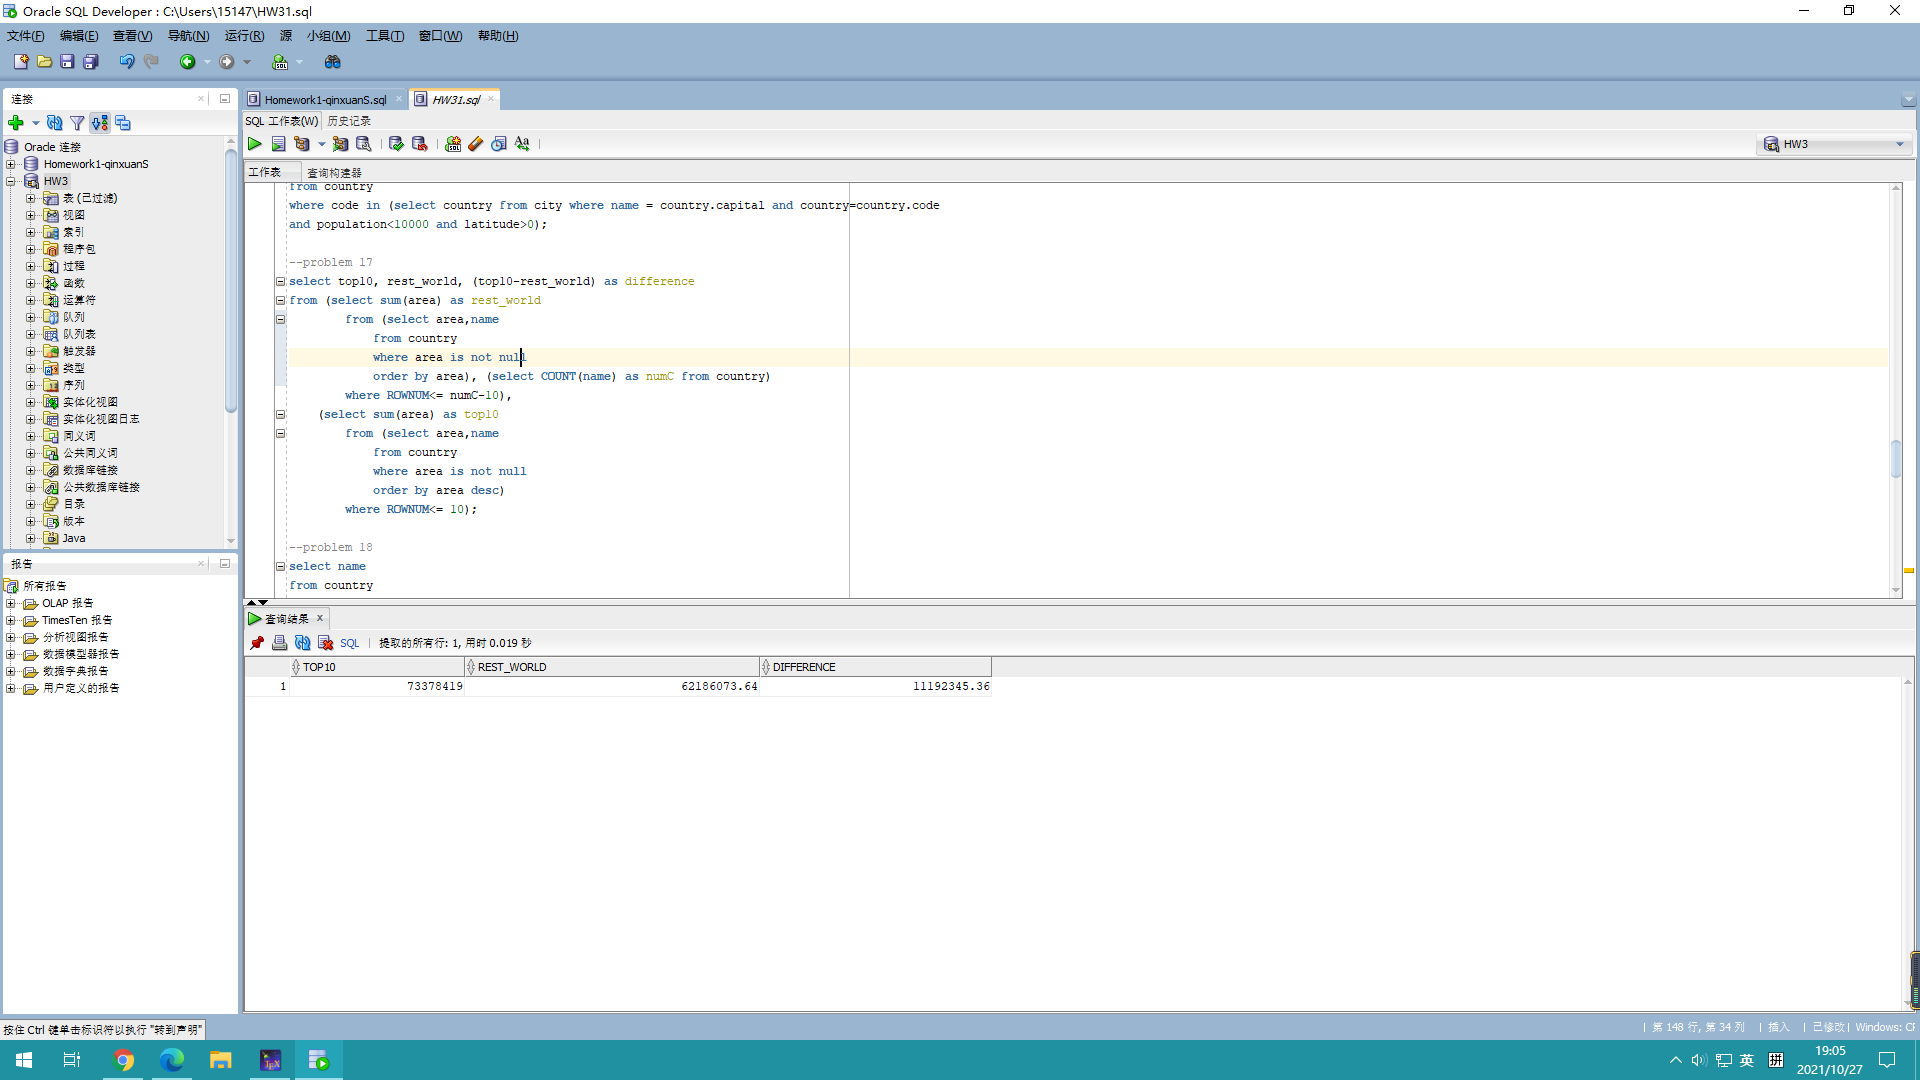
\includegraphics[width=1\linewidth]{../screen/p17}
		\caption{p17}
		\label{fig:p17}
	\end{figure}
	
	\noindent 18. [2 points] Find all countries that cross continental boundaries.   \\
	
	\begin{lstlisting}[language=] 
SELECT name
FROM country
WHERE code in (SELECT country
	FROM encompasses
	GROUP BY country
	HAVING COUNT(continent)>=2);
	\end{lstlisting} 
	Output screen snapshots:
	\begin{figure}[H]
		\centering
		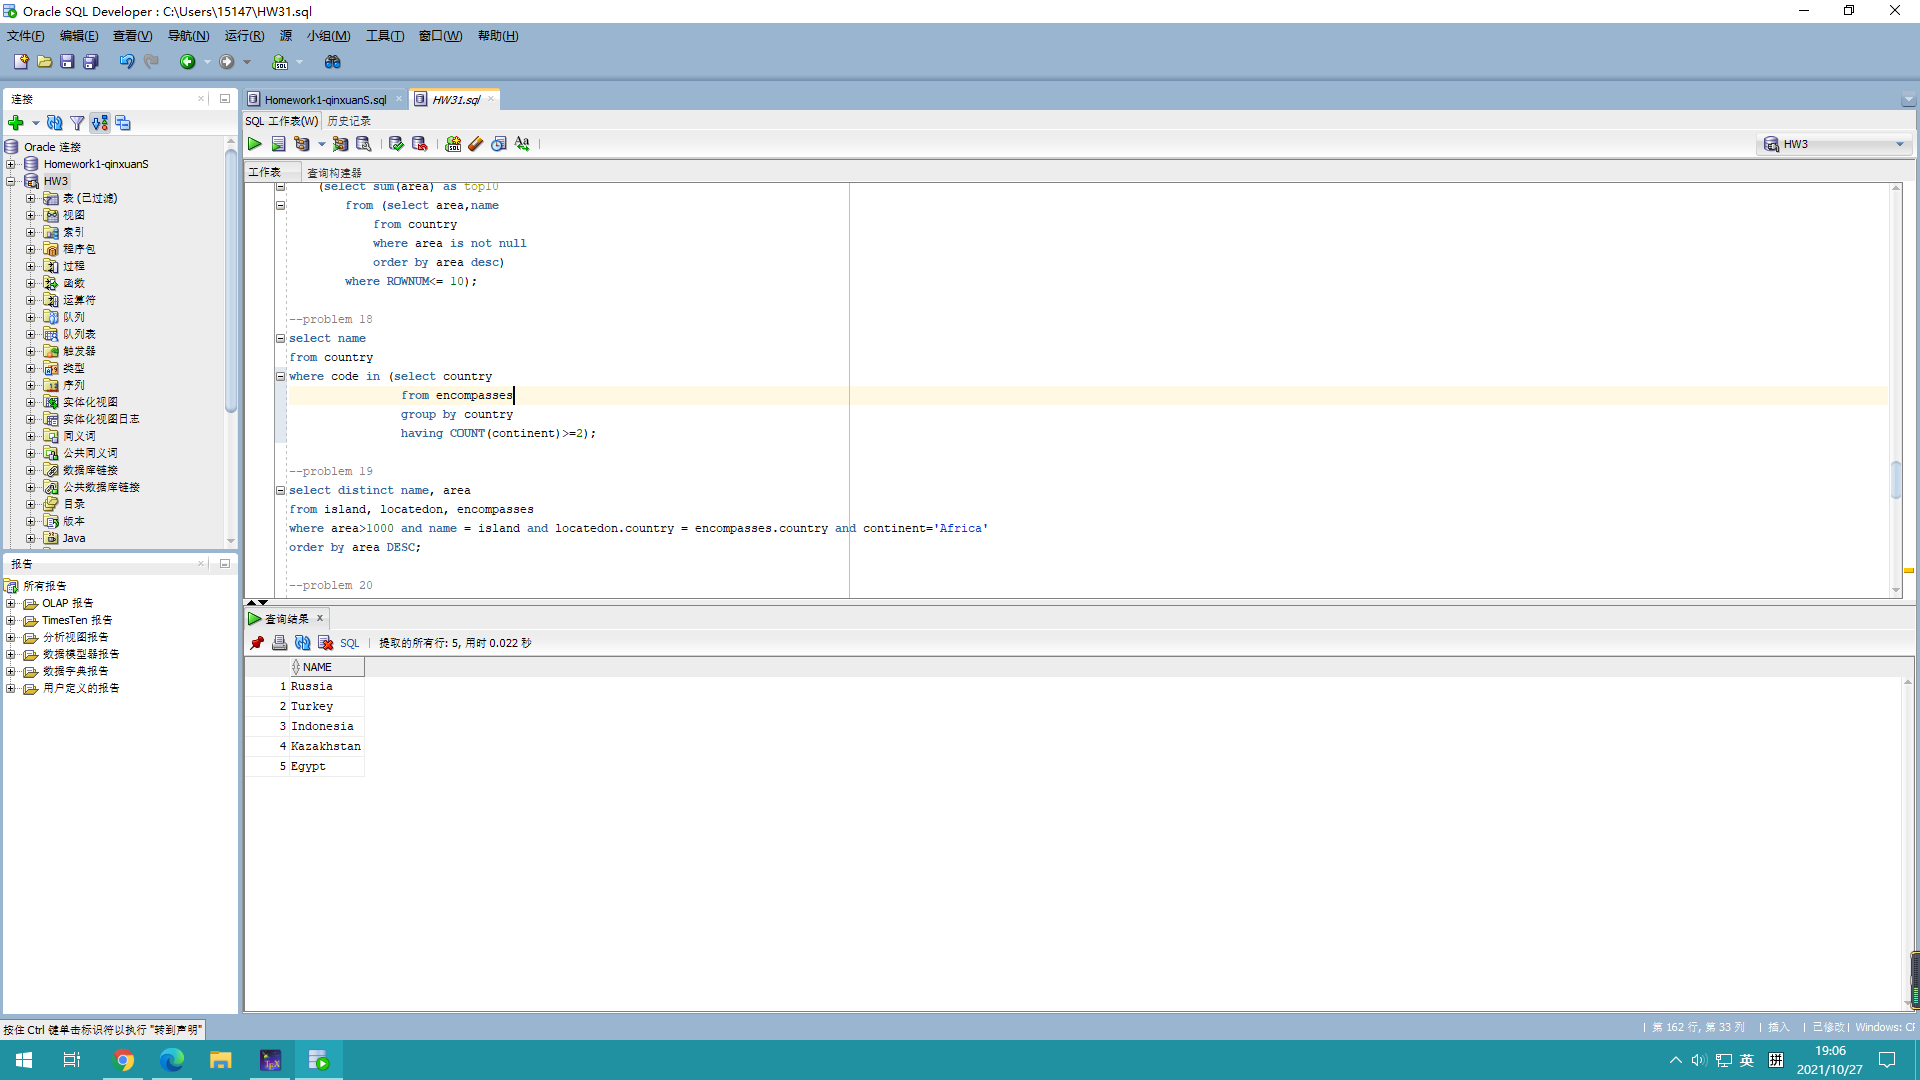
\includegraphics[width=0.9\linewidth]{../screen/p18}
		\caption{p18}
		\label{fig:p18}
	\end{figure}
	
	\noindent 19. [2 points] Display each island in Africa and its area if the area is larger than 1000 square kilometers. The output should be in descending order of the size of the areas.    \\
	
	\begin{lstlisting}[language=] 
SELECT distinct name, area
FROM island, locatedon, encompasses
WHERE area>1000 and name = island and locatedon.country = encompasses.country 
	and continent='Africa'
ORDER BY area DESC;
	\end{lstlisting} 
	Output screen snapshots:
	\begin{figure}[H]
		\centering
		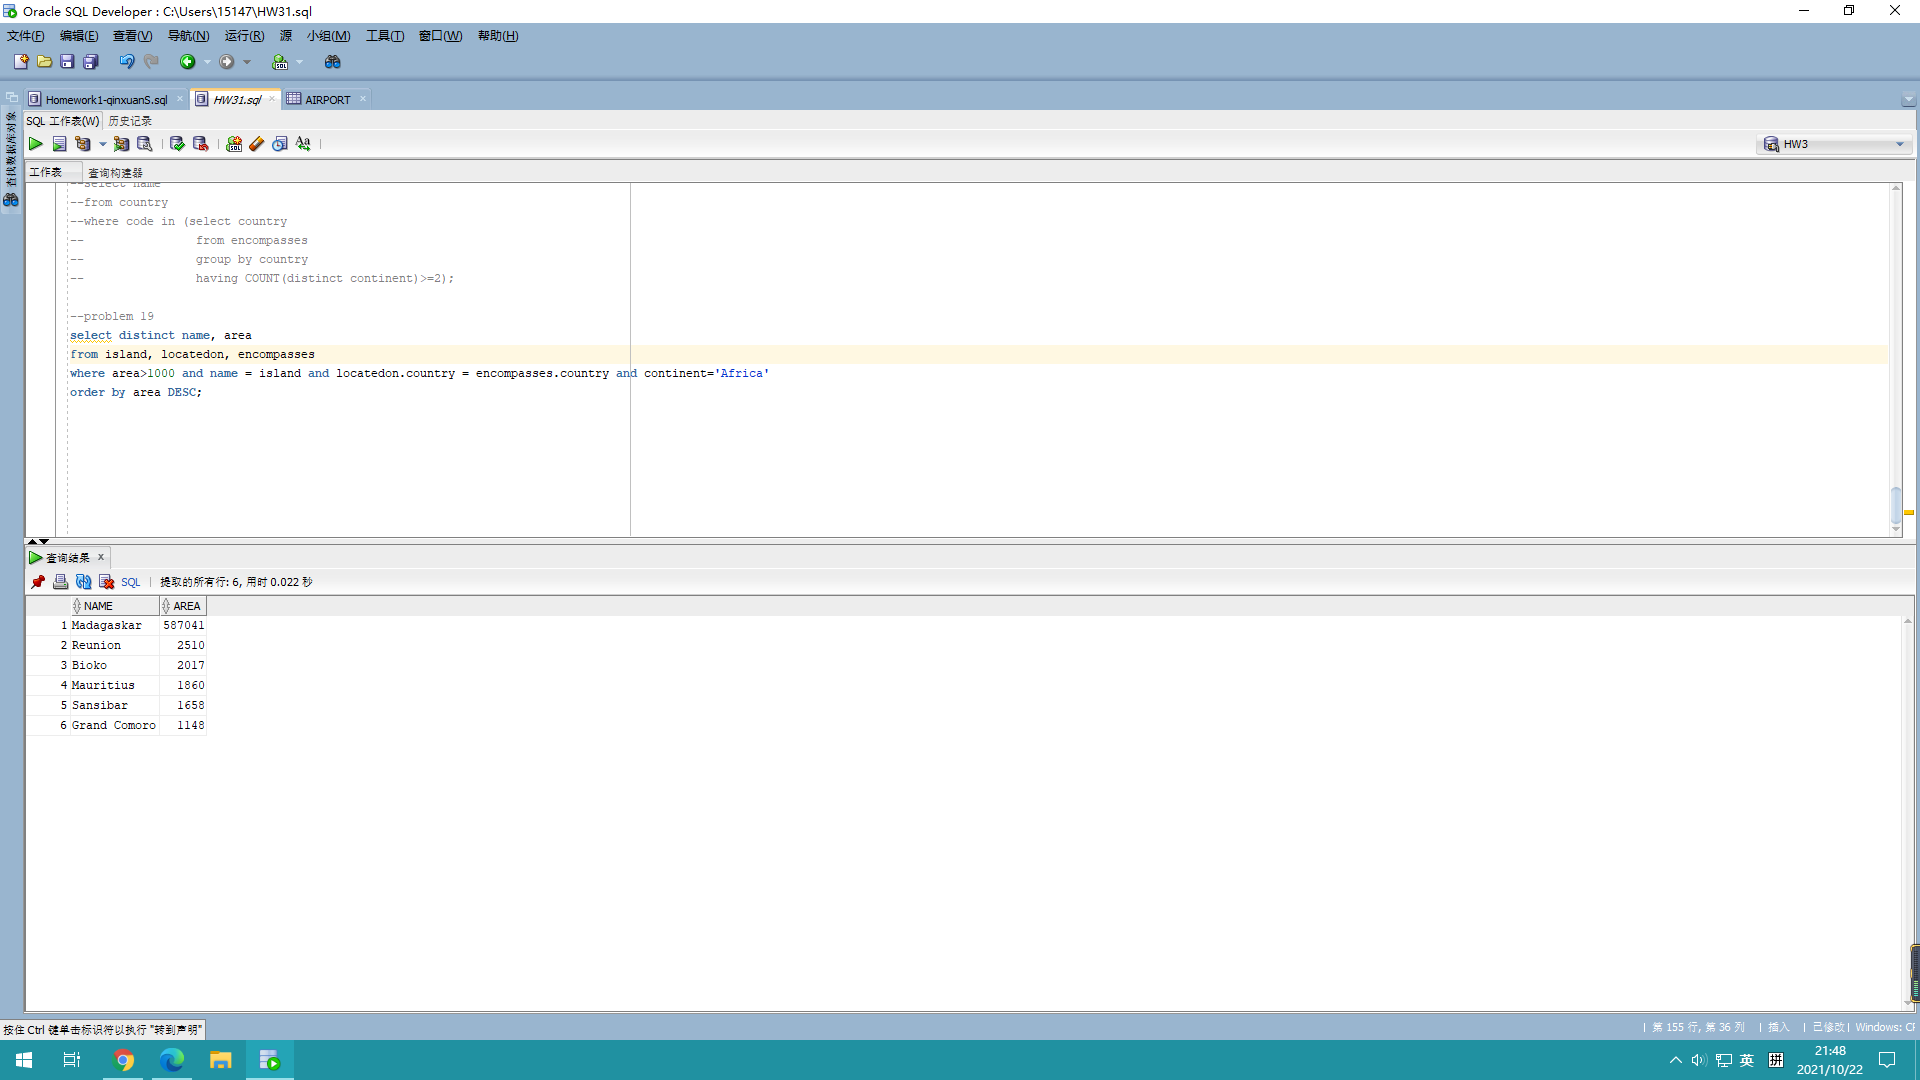
\includegraphics[width=0.9\linewidth]{../screen/p19}
		\caption{p19}
		\label{fig:p19}
	\end{figure}
	
	\noindent 20. [3 points] List the names and GDPs of those countries that are members of the NATO and more than 5 percent of their population are Muslims.   \\
	
	\begin{lstlisting}[language=] 
SELECT name, gdp
FROM country, economy
WHERE country.code = economy.country and country.code in (
	(SELECT country FROM ismember WHERE organization='NATO')
	INTERSECT
	(SELECT country FROM religion WHERE name='Muslim' and percentage>5)
);
	\end{lstlisting} 
	Output screen snapshots:
	\begin{figure}[H]
		\centering
		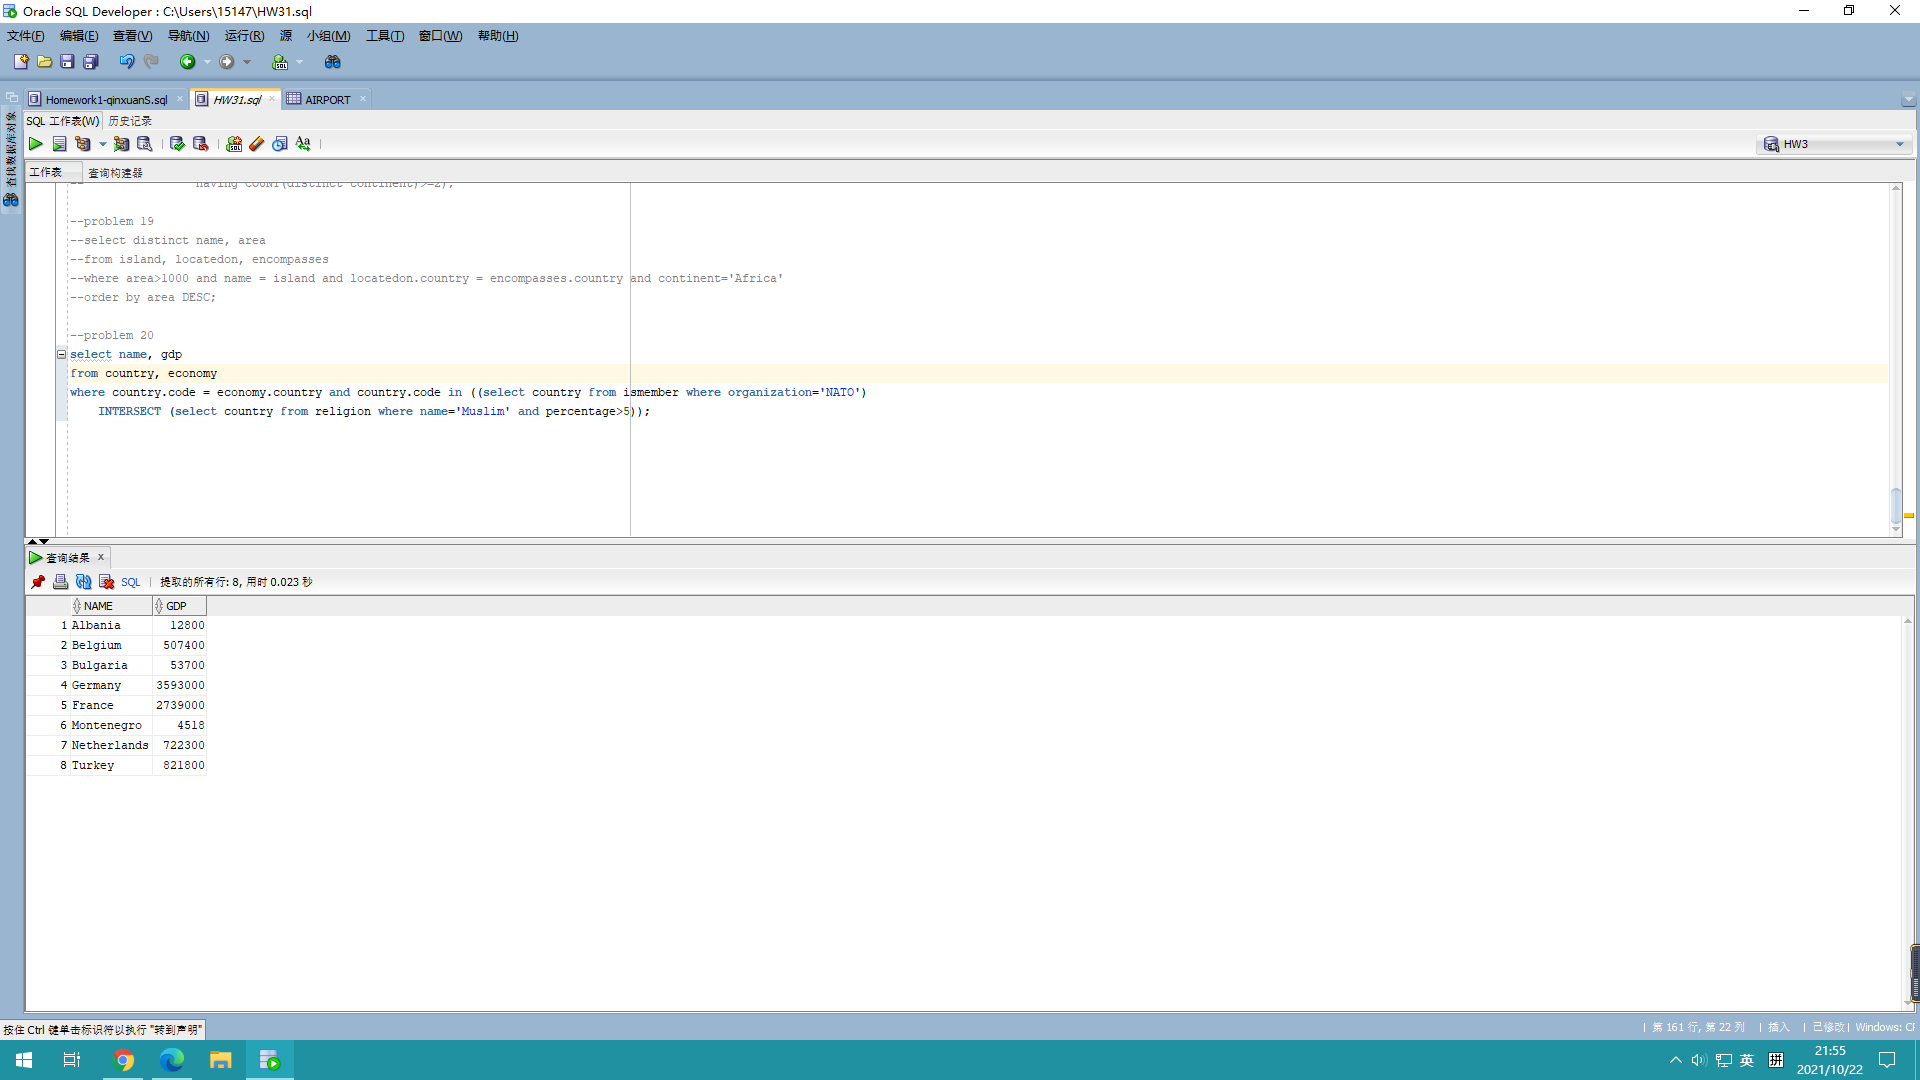
\includegraphics[width=0.7\linewidth]{../screen/p20}
		\caption{p20}
		\label{fig:p20}
	\end{figure}
	
	\noindent 21. [1 point] Find names of rivers which cross at least 12 provinces in the same country.   \\
	
	\begin{lstlisting}[language=] 
SELECT river,country FROM located WHERE river is not null
GROUP BY river,country
HAVING COUNT(province)>=12;
	\end{lstlisting} 
	Output screen snapshots:
	\begin{figure}[H]
		\centering
		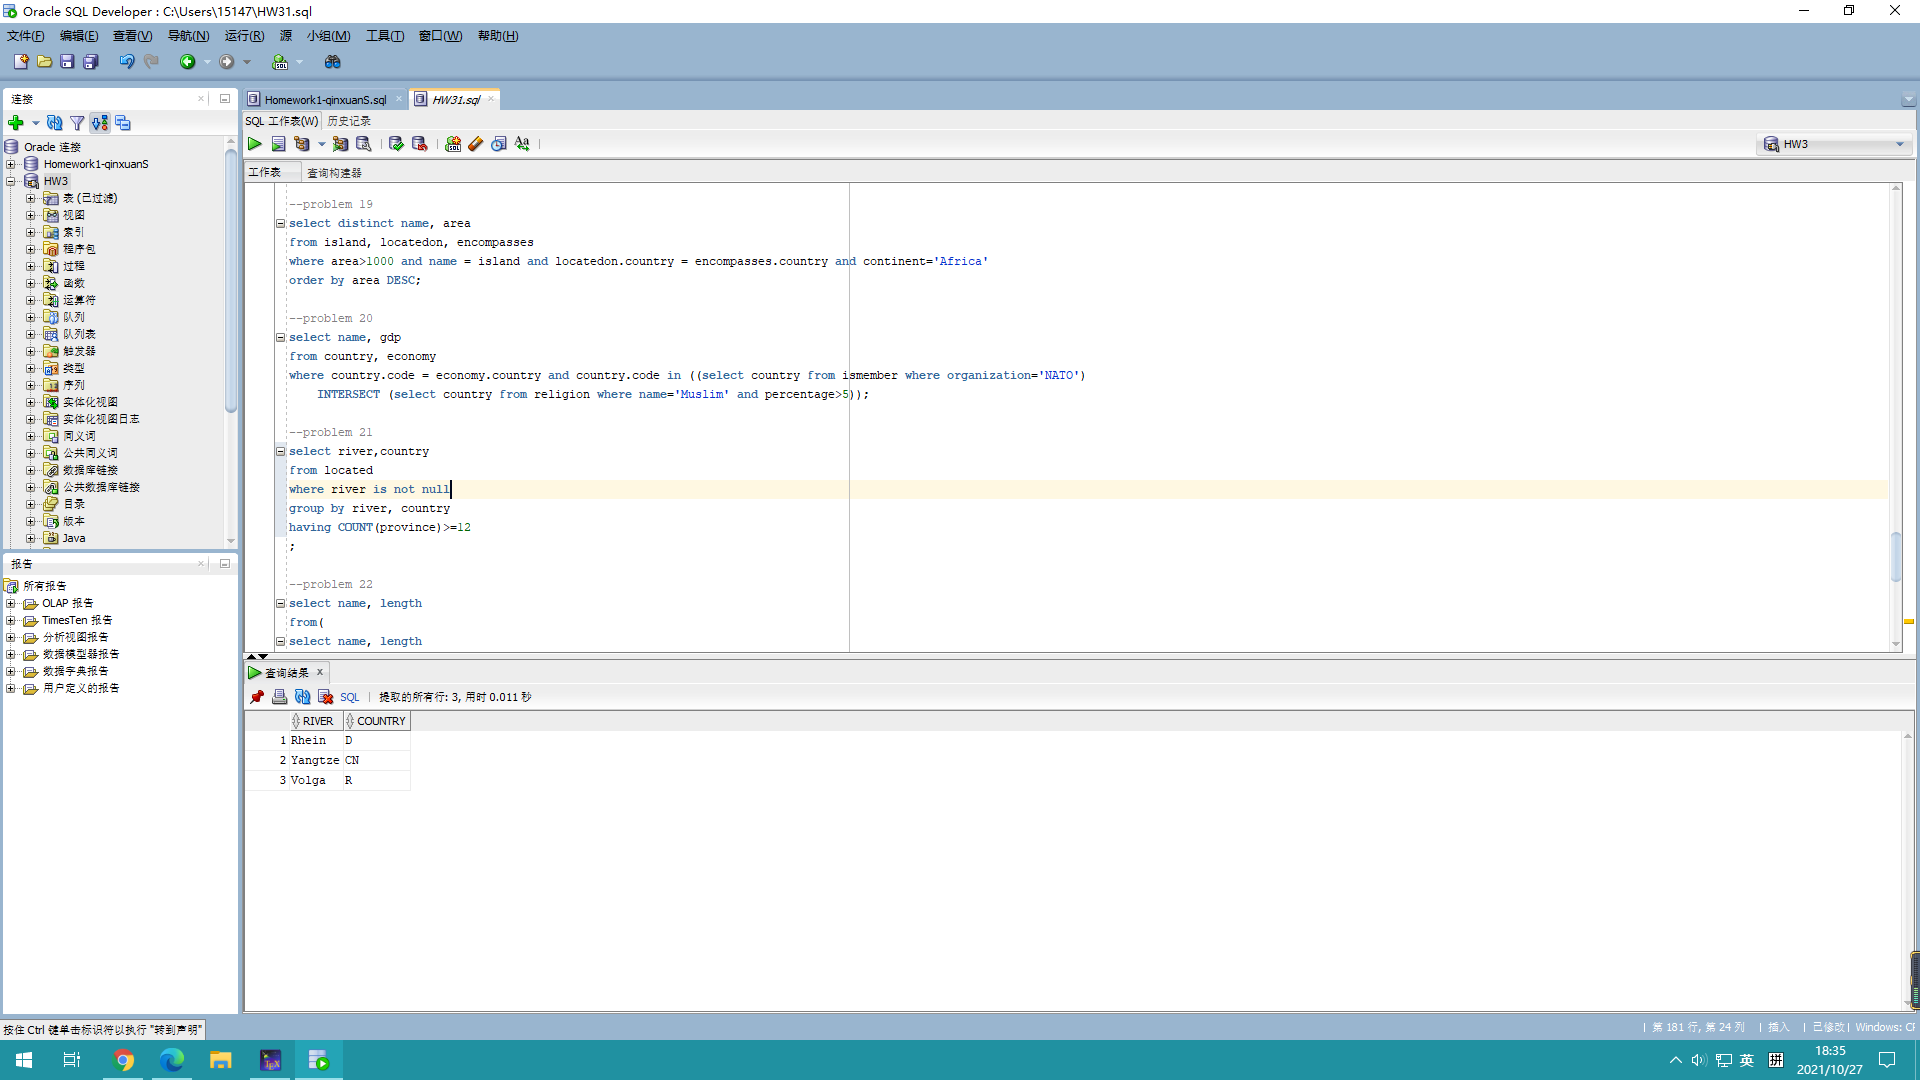
\includegraphics[width=0.7\linewidth]{../screen/p21}
		\caption{p21}
		\label{fig:p21}
	\end{figure}
	
	\noindent 22. [2 points] Find the name and length of the longest river on the American continent.   \\
	
	\begin{lstlisting}[language=] 
SELECT name, length
FROM(
	SELECT name, length
	FROM river
	WHERE name in (
		SELECT river FROM encompasses, located 
		WHERE located.country=encompasses.country and 
			continent='America' and river is not null) )
WHERE length>=(SELECT MAX(length) FROM river
	WHERE name in (SELECT river FROM encompasses, located 
		WHERE located.country=encompasses.country and 
			continent='America' and river is not null) );
	\end{lstlisting} 
	Output screen snapshots:
	\begin{figure}[H]
		\centering
		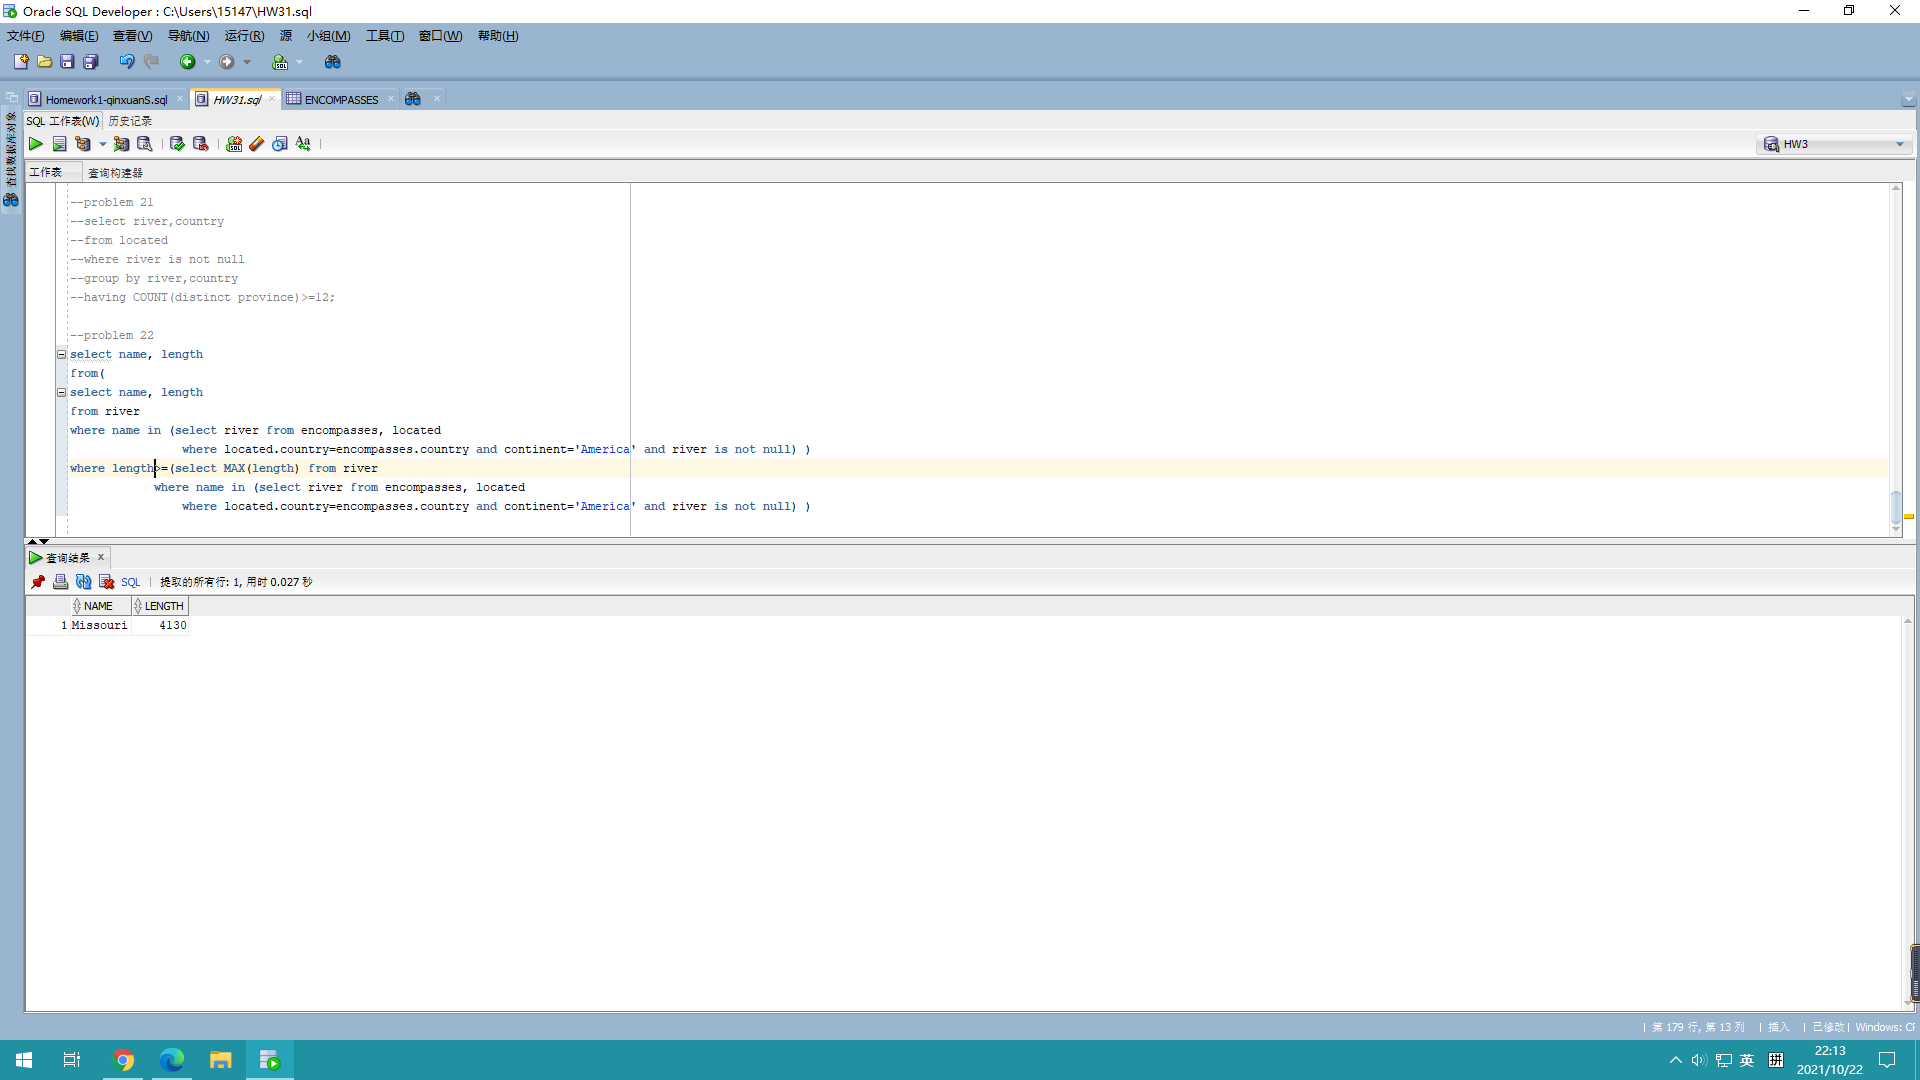
\includegraphics[width=1\linewidth]{../screen/p22}
		\caption{p22}
		\label{fig:p22}
	\end{figure}
	
	\noindent 23. [3 points] Find the provinces that have the largest number of islands in the world. Output the country code, the province, and the number of islands.    \\
	
	\begin{lstlisting}[language=] 
with NumberIsland(country, province, number_of_islands) as
(select country, province, COUNT(island)
	FROM locatedon
	GROUP BY country,province)
SELECT country, province, number_of_islands
FROM NumberIsland
WHERE number_of_islands >= all(SELECT number_of_islands
	FROM NumberIsland);
	\end{lstlisting} 
	Output screen snapshots:
	\begin{figure}[H]
		\centering
		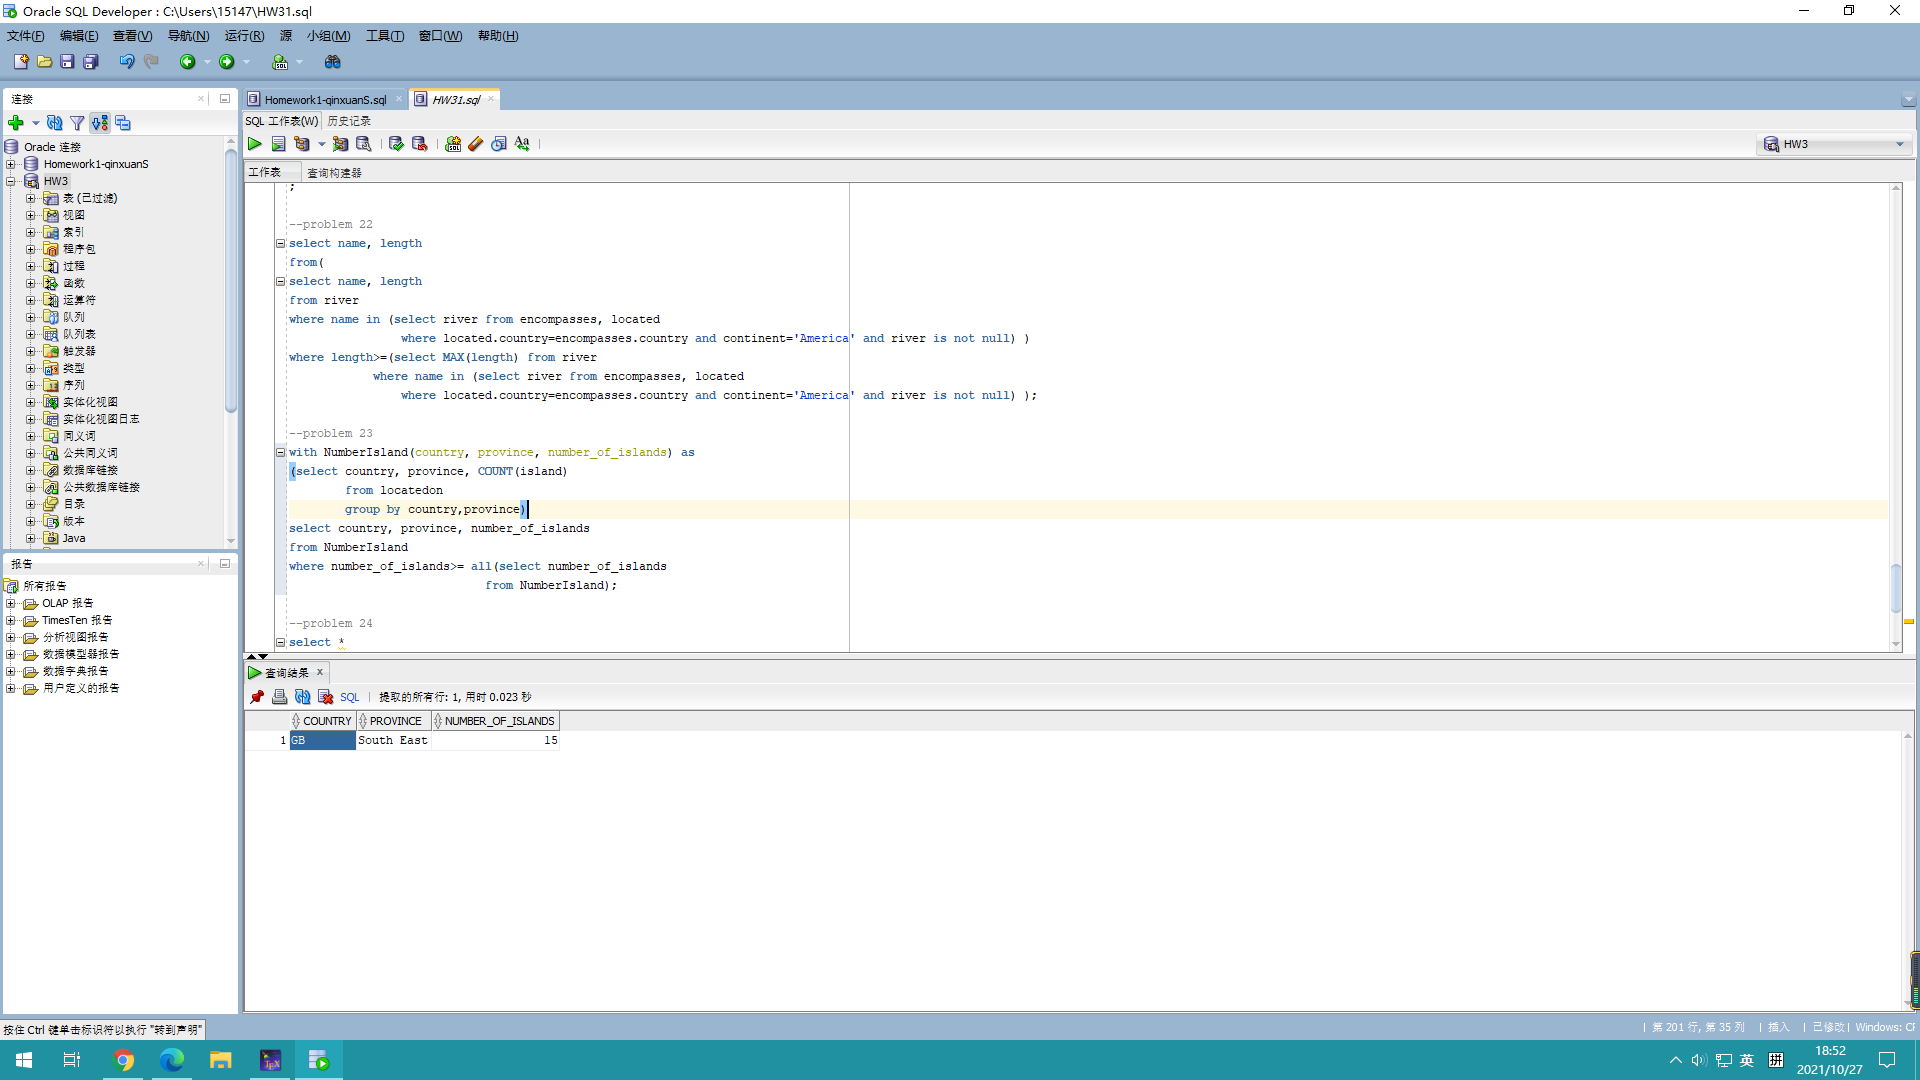
\includegraphics[width=0.87\linewidth]{../screen/p23}
		\caption{p23}
		\label{fig:p23}
	\end{figure}
	
	\noindent 24. [3 points] List the 10 country names (attribute “Country Name”) with the highest population density (attribute “Population Density”) as well as the percentage of the world population (attribute “Percentage”) each one contains.    \\
	
	\begin{lstlisting}[language=] 
SELECT * FROM(
	SELECT name as Country_Name,(population/area) as Population_Density,
	 	(population/total)*100 as Percentage
	FROM country, (SELECT SUM(population) as total FROM country)
	ORDER BY Population_Density DESC)
WHERE rownum<=10;
	\end{lstlisting} 
	Output screen snapshots:
	\begin{figure}[H]
		\centering
		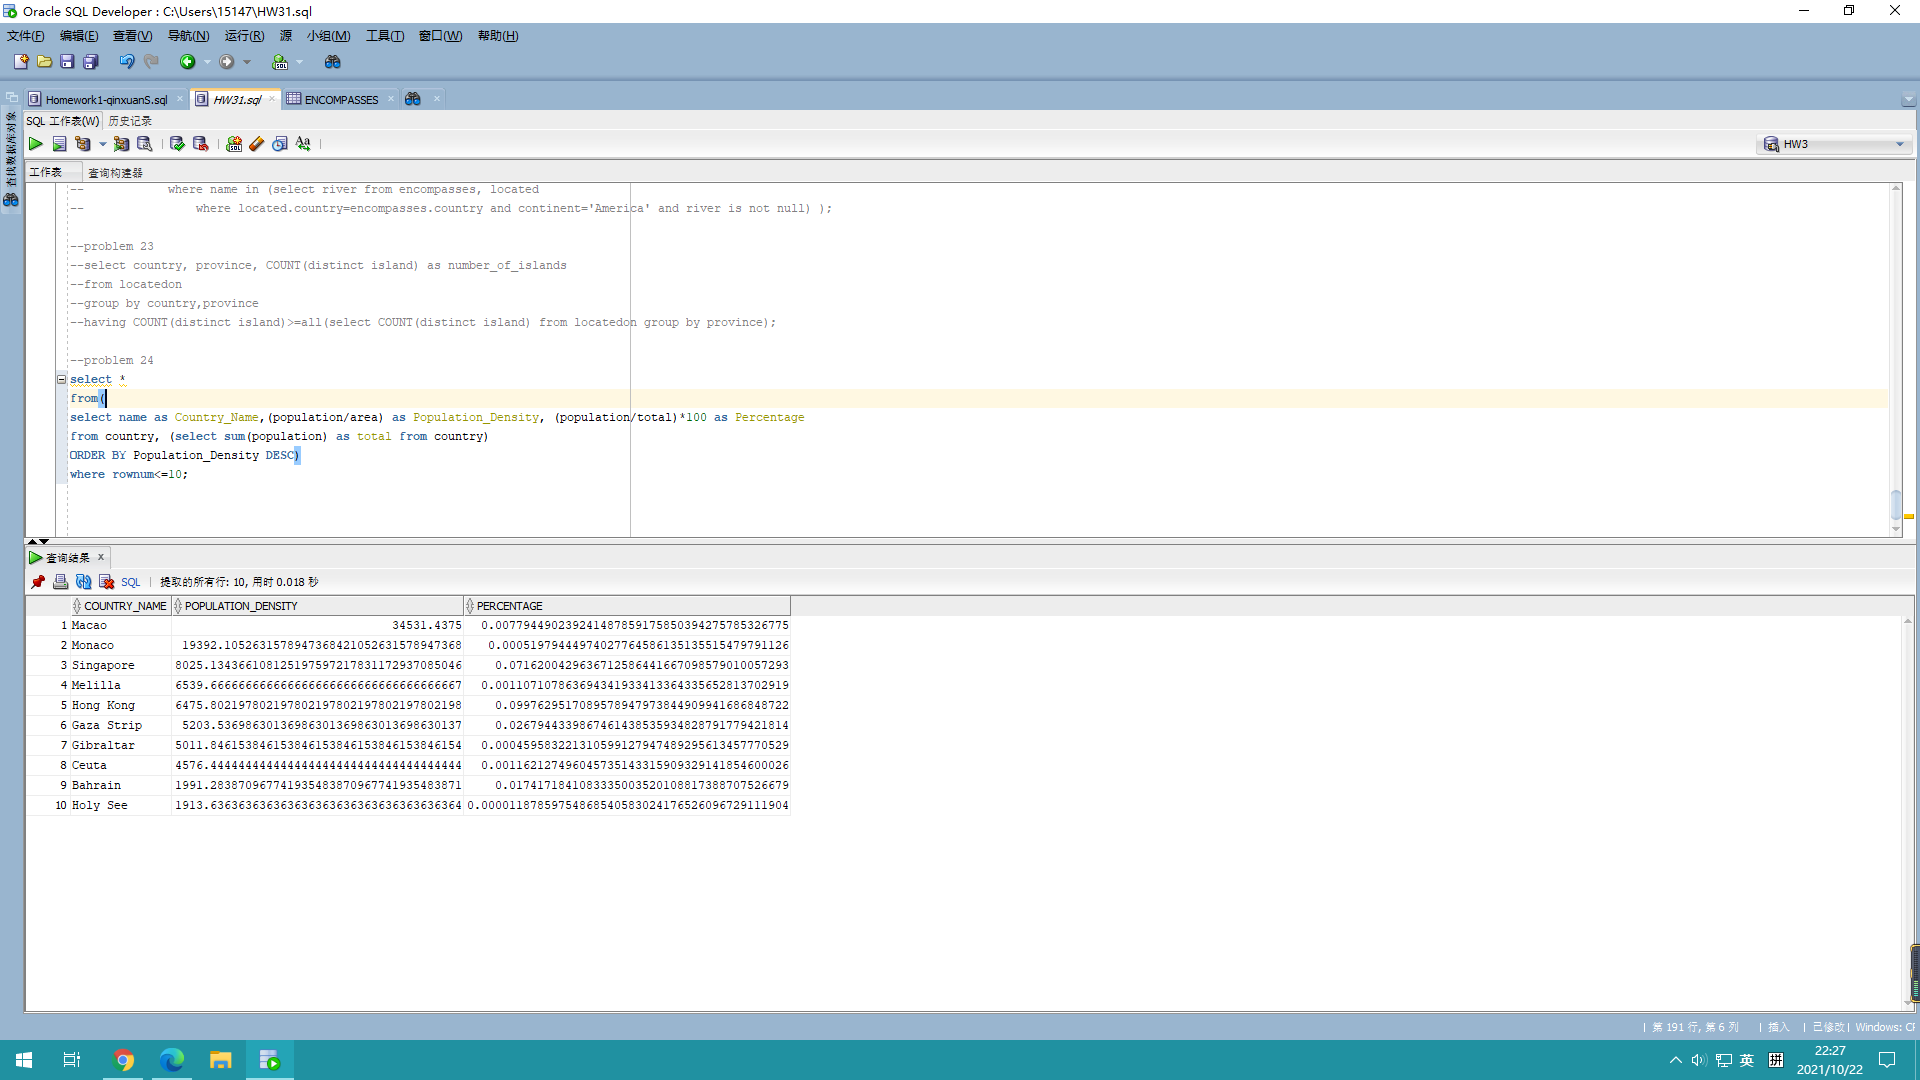
\includegraphics[width=0.87\linewidth]{../screen/p24}
		\caption{p24}
		\label{fig:p24}
	\end{figure}
	
	\noindent 25. [5 points] List the names of organizations that have only Asian countries as members.   \\
	
	\begin{lstlisting}[language=] 
SELECT distinct organization
FROM ismember m
WHERE not exists(
	(SELECT country FROM ismember n WHERE m.organization=n.organization)
	MINUS
	(SELECT country FROM encompasses WHERE continent='Asia')
);
	\end{lstlisting} 
	Output screen snapshots:
	\begin{figure}[H]
		\centering
		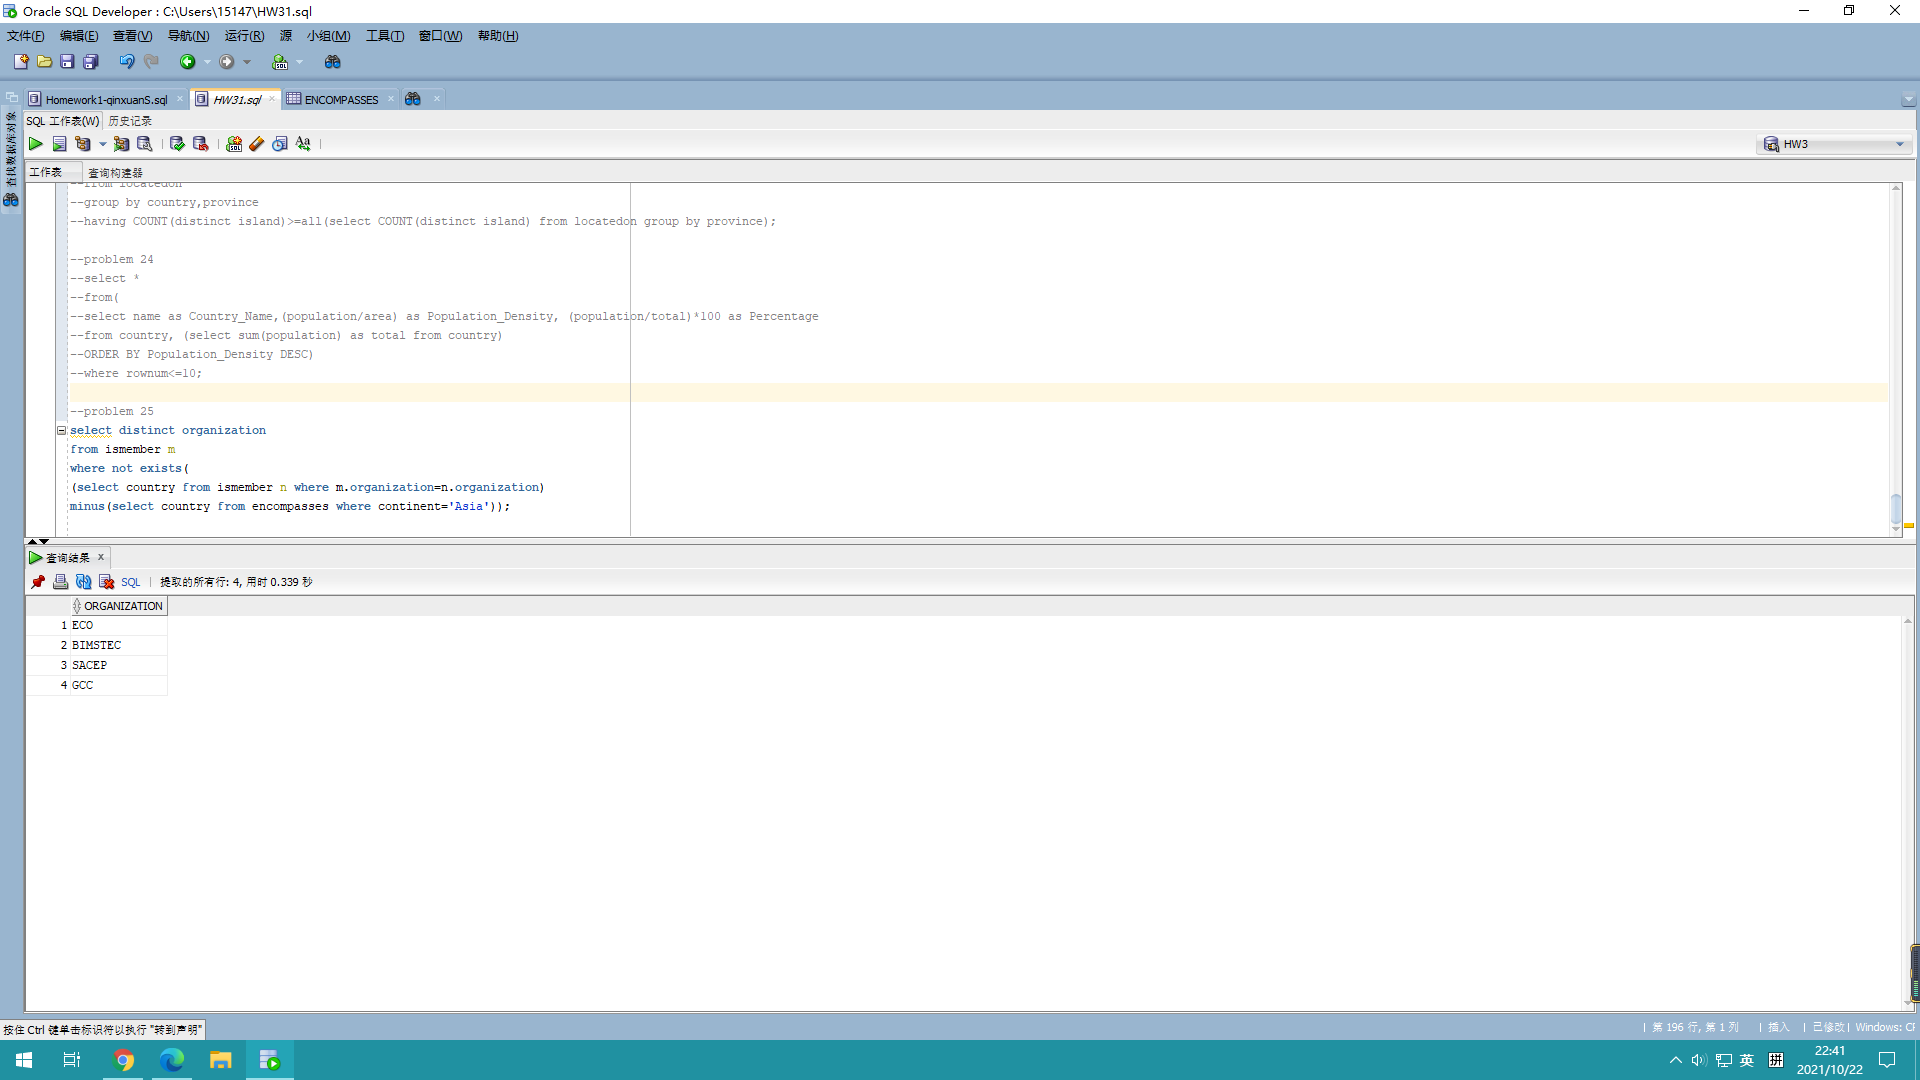
\includegraphics[width=1\linewidth]{../screen/p25}
		\caption{p25}
		\label{fig:p25}
	\end{figure}
	
	\clearpage
	
	\section{Exercise 2}
	
	1. [3 points] Find the names of customers who have booked flights at every company in the US.  \\
	
	\begin{table}[H]
		\begin{tabular}{|l|l|l|l|}
			\hline
			Customer & customerID & name & address \\ \hline
					 &  \_cus     &  P.  &  	   \\ \hline
		\end{tabular}
	\end{table}

	\begin{table}[H]
		\begin{tabular}{|l|l|l|l|l|l|l|}
			\hline
			Book & bID & cID & fnumber & customerID & seat & date \\ \hline
				 & 	   & \_cID1 &      &  G.\_cus	& 	   &  	  \\ \hline
		\end{tabular}
	\end{table}

	\begin{table}[H]
		\begin{tabular}{|l|l|l|l|}
			\hline
			Company & cID & name & location \\ \hline
					& \_cID2 & 	 &   US		\\ \hline
		\end{tabular}
	\end{table}

	\begin{table}[H]
		\begin{tabular}{|c|}
			\hline
			Conditions \\ \hline
			CNT.UN.ALL.\_cID1 = CNT.UN.ALL.\_cID2  \\ \hline
		\end{tabular}
	\end{table}
	
	\noindent 2. [2 points] Find the names and addresses of customers who never booked a flight. \\
	
	\begin{table}[H]
		\begin{tabular}{|l|l|l|l|}
			\hline
			Customer & customerID & name & address \\ \hline
					 &  \_cus     & P.\_n &  P.\_add	\\ \hline
		\end{tabular}
	\end{table}
	
	\begin{table}[H]
		\begin{tabular}{|l|l|l|l|l|l|l|}
			\hline
			Book & bID & cID & fnumber & customerID & seat & date \\ \hline
			$\neg$ &   &     &      &  \_cus	& 	   &  	  \\ \hline
		\end{tabular}
	\end{table}
	
	\noindent 3. [2 points] Find the names of customers who booked the flight to New York more than once.   \\
	
	\begin{table}[H]
		\begin{tabular}{|l|l|l|l|}
			\hline
			Customer & customerID & name & address \\ \hline
					 &  \_cus     & P.   &      	\\ \hline
		\end{tabular}
	\end{table}
	
	\begin{table}[H]
		\begin{tabular}{|l|l|l|l|l|l|l|}
			\hline
			Book & bID & cID & fnumber & customerID & seat & date \\ \hline
				 &     &     & \_fn1   &  \_cus	    & 	   & \_date 	  \\ \hline
				 &     &     & \_fn2   &  \_cus	    & 	   & $\neg$\_date 	  \\ \hline
		\end{tabular}
	\end{table}

	\begin{table}[H]
		\begin{tabular}{|l|l|l|l|l|l|l|}
			\hline
			Flight & cID & fnumber & departure & arrival & price & numberOfSeats \\ \hline
				   &  	 &  \_fn1  &  		   & New York &  	 &  			 \\ \hline
			 	   &  	 &  \_fn2  &  		   & New York &  	 &  			 \\ \hline
		\end{tabular}
	\end{table}
	
	\noindent 4. [3 points] Find the names of the companies that have the biggest (in terms of the number of seats) airplane.  \\
	
	\begin{table}[H]
		\begin{tabular}{|l|l|l|l|l|l|l|}
			\hline
			Flight & cID & fnumber & departure & arrival & price & numberOfSeats \\ \hline
				   & \_cID1  &  		&  			&  		&  		 &  	\_numS		 \\ \hline
			$\neg$ & \_cID2  &  		&  			&  		&  		 &  	$>$\_numS		 \\ \hline
		\end{tabular}
	\end{table}
	
	\begin{table}[H]
		\begin{tabular}{|l|l|l|l|}
			\hline
			Company & cID & name & location \\ \hline
					& \_cID1 &  P. &  		\\ \hline
		\end{tabular}
	\end{table}
	
	\noindent 5. [2 points] Find the names of customers who booked flights to Boston and Seattle.  \\
	
	\begin{table}[H]
		\begin{tabular}{|l|l|l|l|l|l|l|}
			\hline
			Book & bID & cID & fnumber & customerID & seat & date \\ \hline
				 & 	   & \_cID1	 &  \_fn1 &	\_cus	&  		&  		\\ \hline
			 	 & 	   & \_cID2	 &  \_fn2 &	\_cus	&  		&  		\\ \hline
		\end{tabular}
	\end{table}
	
	\begin{table}[H]
		\begin{tabular}{|l|l|l|l|l|l|l|}
			\hline
			Flight & cID & fnumber & departure & arrival & price & numberOfSeats \\ \hline
				   & \_cID1	 &  \_fn1 & 		 &  Boston	& 	 &  				\\ \hline
			   	   & \_cID2	 &  \_fn2 & 		 &  Seattle	& 	 &  				\\ \hline
		\end{tabular}
	\end{table}
	
	\noindent 6. [3 points] Insert tuples into a new table CustomerCheck that stores the names and addresses of customers along with their flight numbers who booked a flight from New York to LA on 09/30/21.  \\
	
	\begin{table}[H]
		\begin{tabular}{|l|l|l|l|}
			\hline
			Customer & customerID & name & address \\ \hline
					 &  \_cus	  & \_n  & \_add   \\ \hline
		\end{tabular}
	\end{table}
	
	\begin{table}[H]
		\begin{tabular}{|l|l|l|l|l|l|l|}
			\hline
			Book & bID & cID & fnumber & customerID & seat & date \\ \hline
				 & 	   & \_cID & \_fn  &  \_cus     &	  & 09/30/21	 \\ \hline
		\end{tabular}
	\end{table}
	
	\begin{table}[H]
		\begin{tabular}{|l|l|l|l|l|l|l|}
			\hline
			Flight & cID & fnumber & departure & arrival & price & numberOfSeats \\ \hline
				   & \_cID & \_fn  &  New York &  LA  	 & 		 & 				 \\ \hline
		\end{tabular}
	\end{table}

	\begin{table}[H]
		\begin{tabular}{|c|l|l|l|}
			\hline
			CustomerCheck & name & address & fnumber \\ \hline
				I.		  &  \_n  & \_add  & \_fn   \\ \hline
		\end{tabular}
	\end{table}
	
\end{document}
